%%=============================================================================
%% LaTeX sjabloon voor bachelorproef, HoGent Bedrijf en Organisatie
%% Opleiding Toegepaste Informatica
%%=============================================================================

\documentclass[fleqn,a4paper,12pt]{book}

%%=============================================================================
%% LaTeX sjabloon voor de bachelorproef, HoGent Bedrijf en Organisatie
%% Opleiding toegepaste informatica
%%
%% Structuur en algemene vormgeving. Meestal hoef je hier niets te wijzigen.
%%
%% Vormgeving gebaseerd op "The Legrand Orange Book", version 2.0 (9/2/15)
%% door Mathias Legrand (legrand.mathias@gmail.com) met aanpassingen door
%% Vel (vel@latextemplates.com). Het oorspronkelijke template is te vinden op
%% http://www.LaTeXTemplates.com
%%
%% Aanpassingen voor HoGent toegepaste informatica:
%%   Bert Van Vreckem <bert.vanvreckem@hogent.be>
%% Licentie:
%%   CC BY-NC-SA 3.0 (http://creativecommons.org/licenses/by-nc-sa/3.0/)
%%=============================================================================

%%-----------------------------------------------------------------------------
%% Packages
%%-----------------------------------------------------------------------------

\usepackage[top=3cm,bottom=3cm,left=3cm,right=3cm,headsep=10pt,a4paper]{geometry} % Page margins
\usepackage[utf8]{inputenc}  % Accenten gebruiken in tekst (vb. é ipv \'e)
\usepackage{amsfonts}        % AMS math packages: extra wiskundige
\usepackage{amsmath}         %   symbolen (o.a. getallen-
\usepackage{amssymb}         %   verzamelingen N, R, Z, Q, etc.)
\usepackage[english,dutch]{babel}    % Taalinstellingen: woordsplitsingen,
                             %  commando's voor speciale karakters
                             %  ("dutch" voor NL)
\usepackage{iflang}
\usepackage{eurosym}         % Euro-symbool €
\usepackage{geometry}
\usepackage{graphicx}        % Invoegen van tekeningen
\graphicspath{{img/}}       % Specifies the directory where pictures are stored
\usepackage{tikz}            % Required for drawing custom shapes
\usepackage[pdftex,bookmarks=true]{hyperref}
                             % PDF krijgt klikbare links & verwijzingen,
                             %  inhoudstafel
\usepackage{enumitem}        % Customize lists
\setlist{nolistsep}         % Reduce spacing between list items
\usepackage{listings}        % Broncode mooi opmaken
\usepackage{multirow}        % Tekst over verschillende cellen in tabellen
\usepackage{rotating}        % Tabellen en figuren roteren

\usepackage{booktabs}        % Required for nicer horizontal rules in tables

\usepackage{xcolor}          % Required for specifying colors by name
\definecolor{maincolor}{RGB}{0,147,208} % Define the main color used for
                             % highlighting throughout the book
                             % 0, 147, 208 = officiële kleur HoGent FBO

% Paragraph style: no indent, add space between paragraphs
\setlength{\parindent}{0em}
\setlength{\parskip}{1em}

\usepackage{etoolbox}
\usepackage{titling} % Macros for title, author, etc
\usepackage{lipsum}          % Voor vultekst (lorem ipsum)

\usepackage{cleveref}        % Reference labels by name
\usepackage[acronym]{glossaries}

\usepackage{tabularx}
\usepackage{booktabs}
\usepackage{makecell}

\usepackage{float,lscape}
\usepackage{pdflscape}

% Table style
\renewcommand\theadalign{bc}
\renewcommand\theadfont{\bfseries}
\renewcommand\theadgape{\Gape[4pt]}
\renewcommand\cellgape{\Gape[4pt]}
\renewcommand{\arraystretch}{2}

% TODOs
\newcommand{\TODO}{}

%----------------------------------------------------------------------------------------
%	FONTS
%----------------------------------------------------------------------------------------

\usepackage{avant} % Use the Avantgarde font for headings
%\usepackage{times} % Use the Times font for headings
\usepackage{mathptmx} % Use the Adobe Times Roman as the default text font together with math symbols from the Sym­bol, Chancery and Com­puter Modern fonts

\usepackage{microtype} % Slightly tweak font spacing for aesthetics
\usepackage[utf8]{inputenc} % Required for including letters with accents
\usepackage[T1]{fontenc} % Use 8-bit encoding that has 256 glyphs

%------------------------------------------------------------------------------
%	TITLE PAGE
%------------------------------------------------------------------------------

\newcommand{\inserttitlepage}{%
\begin{titlepage}
  \newgeometry{top=2cm,bottom=1.5cm,left=1.5cm,right=1.5cm}
  \begin{center}

    \begingroup
    \rmfamily
    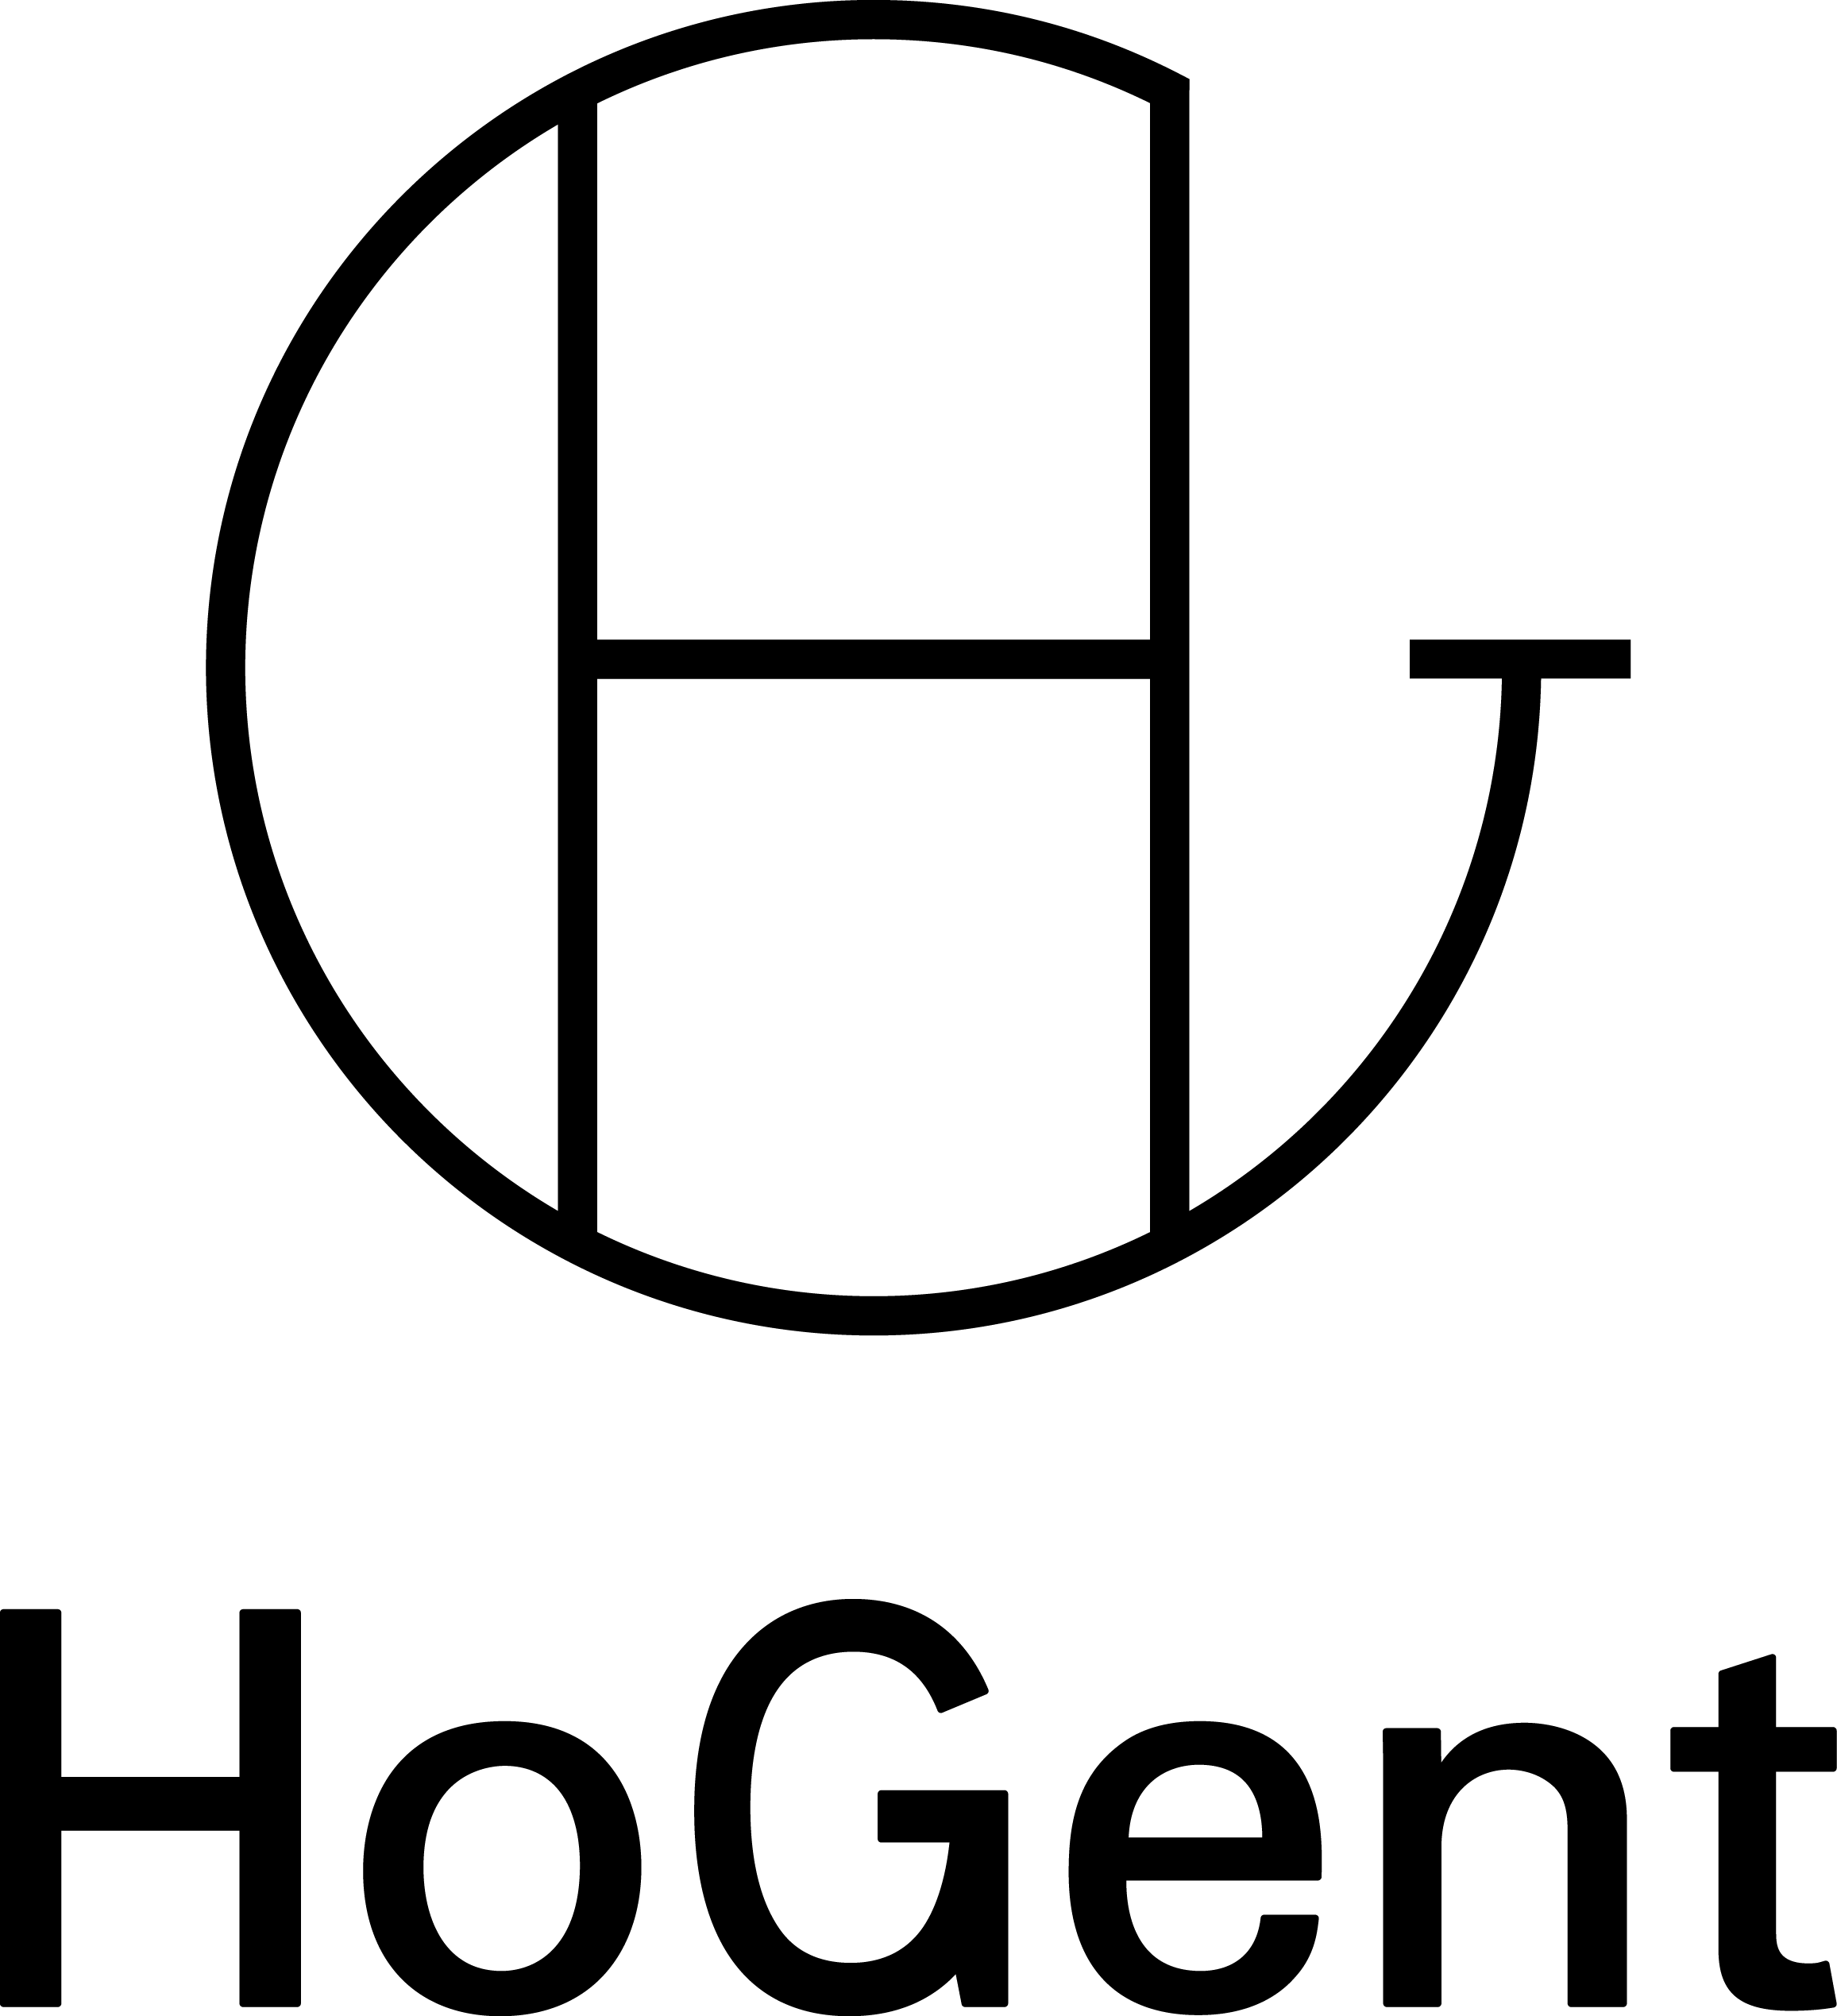
\includegraphics[width=2.5cm]{img/HG-beeldmerk-woordmerk}\\[.5cm]
    Faculteit Bedrijf en Organisatie\\[3cm]
    \titel
    \vfill
    \student\\[3.5cm]
    Scriptie voorgedragen tot het bekomen van de graad van\\professionele bachelor in de toegepaste informatica\\[2cm]
    Promotor:\\
    \promotor\\
    \ifdefempty{\copromotor}{\vspace{2.5cm}}{Co-promotor:\\\copromotor\\[2.5cm]}
    Instelling: \instelling\\[.5cm]
    Academiejaar: \academiejaar\\[.5cm]
    \ifcase \examenperiode \or Eerste \or Tweede \else Derde \fi examenperiode
    \endgroup

  \end{center}
  \restoregeometry
\end{titlepage}
  \emptypage
\begin{titlepage}
  \newgeometry{top=5.35cm,bottom=1.5cm,left=1.5cm,right=1.5cm}
  \begin{center}

    \begingroup
    \rmfamily
    \IfLanguageName{dutch}{Faculteit Bedrijf en Organisatie}{Faculty of Business and Information Management}\\[3cm]
    \titel
    \vfill
    \student\\[3.5cm]
    \IfLanguageName{dutch}{Scriptie voorgedragen tot het bekomen van de graad van\\professionele bachelor in de toegepaste informatica}{Thesis submitted in partial fulfilment of the requirements for the degree of\\professional bachelor of applied computer science}\\[2cm]
    Promotor:\\
    \promotor\\
    \ifdefempty{\copromotor}{\vspace{2.5cm}}{Co-promotor:\\\copromotor\\[2.5cm]}
    \IfLanguageName{dutch}{Instelling}{Institution}: \instelling\\[.5cm]
    \IfLanguageName{dutch}{Academiejaar}{Academic year}: \academiejaar\\[.5cm]
    \IfLanguageName{dutch}{%
    \ifcase \examenperiode \or Eerste \or Tweede \else Derde \fi examenperiode}{%
    \ifcase \examenperiode \or First \or Second \else Third \fi examination period}
    \endgroup

  \end{center}
  \restoregeometry
\end{titlepage}
}

%----------------------------------------------------------------------------------------
%	BIBLIOGRAPHY AND INDEX
%----------------------------------------------------------------------------------------

\usepackage[style=apa,backend=biber]{biblatex}
\usepackage{csquotes}
\DeclareLanguageMapping{dutch}{dutch-apa}
\addbibresource{bibliography.bib} % BibTeX bibliography file
\addbibresource{../proposal/biblio.bib}
\defbibheading{bibempty}{}

\usepackage{calc} % For simpler calculation - used for spacing the index letter headings correctly
\usepackage{makeidx} % Required to make an index
\makeindex % Tells LaTeX to create the files required for indexing

%----------------------------------------------------------------------------------------
%	MAIN TABLE OF CONTENTS
%----------------------------------------------------------------------------------------

\usepackage{titletoc} % Required for manipulating the table of contents

\contentsmargin{0cm} % Removes the default margin

% Part text styling
\titlecontents{part}[0cm]
{\addvspace{20pt}\centering\large\bfseries}
{}
{}
{}

% Chapter text styling
\titlecontents{chapter}[1.25cm] % Indentation
{\addvspace{12pt}\large\sffamily\bfseries} % Spacing and font options for chapters
{\color{maincolor!60}\contentslabel[\Large\thecontentslabel]{1.25cm}\color{maincolor}} % Chapter number
{\color{maincolor}}
{\color{maincolor!60}\normalsize\;\titlerule*[.5pc]{.}\;\thecontentspage} % Page number

% Section text styling
\titlecontents{section}[1.25cm] % Indentation
{\addvspace{3pt}\sffamily\bfseries} % Spacing and font options for sections
{\contentslabel[\thecontentslabel]{1.25cm}} % Section number
{}
{\hfill\color{black}\thecontentspage} % Page number
[]

% Subsection text styling
\titlecontents{subsection}[1.25cm] % Indentation
{\addvspace{1pt}\sffamily\small} % Spacing and font options for subsections
{\contentslabel[\thecontentslabel]{1.25cm}} % Subsection number
{}
{\ \titlerule*[.5pc]{.}\;\thecontentspage} % Page number
[]

% Glossary and list of abbreviations
\newglossaryentry{clustering}{
  name = $clustering$,
  description = {The horizontal scaling ability of a distributed data store over multiple hosts and the interactions within the network between the cluster nodes},
}

\newglossaryentry{datastore}{
  name = $data store$,
  description = A repository of persistently stored and managed collections of data,
}

\newglossaryentry{database}{
  name = $database$,
  description = A data store managed by an database management system,
}

\newglossaryentry{dbms}{
  name = $database management system$,
  description = {Software that manages storage, querying and manipulation of data in a database},
}

\newglossaryentry{cap-theorem}{
  name = $CAP theorem$,
  description = {The proposition that states that a distributed database cannot provide more than two out of three of the CAP guarantees: Consistency, Availability, Partition tolerance},
}

\newglossaryentry{impedance-mismatch}{
name = $Impedance Mismatch$,
description = {The difference between the relational model and the data structures provided by the programming language},
}

\newglossaryentry{newsql}{
  name = $NewSQL$,
  description = {Classification of modern relational database that aims to provide solutions to the scalability and flexibility similar to NoSQL systems, while still maintaining ACID guarantees},
}

\newglossaryentry{nosql}{
  name = $NoSQL$,
  description = {Not Only SQL, classification of modern non-relational database that focuses on horizontal scalability and flexibility in data model},
}

\newglossaryentry{polyglot-persistence}{
  name = $Polyglot Persistence$,
  description = {The practice of using multiple databases to store different types of information},
}

\newglossaryentry{restful}{
  name = $RESTful$,
  description = {Conforming to the REST architecture},
}

\newglossaryentry{sharding}{
  name = $sharding$,
  description = {Distributing of the dataset within a distributed data store, based on certain criteria within the data itself},
}

\newacronym{rdbms}{RDBMS}{Relational Database Management System}
\newacronym{erd}{ERD}{Entity Relationship Diagram}
\newacronym{acid}{ACID}{Atomicity, Consistency, Isolation, Durability}
\newacronym{base}{BASE}{Basically Available, Soft state, Eventual consistency}
\newacronym{rdf}{RDF}{Resource Description Framework}
\newacronym{oltp}{OLTP}{Online Transaction Processing}

\makeglossaries

% List of figures
\titlecontents{figure}[0em]
{\addvspace{-5pt}\sffamily}
{\thecontentslabel\hspace*{1em}}
{}
{\ \titlerule*[.5pc]{.}\;\thecontentspage}
[]

% List of tables
\titlecontents{table}[0em]
{\addvspace{-5pt}\sffamily}
{\thecontentslabel\hspace*{1em}}
{}
{\ \titlerule*[.5pc]{.}\;\thecontentspage}
[]

%----------------------------------------------------------------------------------------
%	MINI TABLE OF CONTENTS IN PART HEADS
%----------------------------------------------------------------------------------------

% Chapter text styling
\titlecontents{lchapter}[0em] % Indenting
{\addvspace{15pt}\large\sffamily\bfseries} % Spacing and font options for chapters
{\color{maincolor}\contentslabel[\Large\thecontentslabel]{1.25cm}\color{maincolor}} % Chapter number
{}
{\color{maincolor}\normalsize\sffamily\bfseries\;\titlerule*[.5pc]{.}\;\thecontentspage} % Page number

% Section text styling
\titlecontents{lsection}[0em] % Indenting
{\sffamily\small} % Spacing and font options for sections
{\contentslabel[\thecontentslabel]{1.25cm}} % Section number
{}
{}

% Subsection text styling
\titlecontents{lsubsection}[.5em] % Indentation
{\normalfont\footnotesize\sffamily} % Font settings
{}
{}
{}

%----------------------------------------------------------------------------------------
%	PAGE HEADERS
%----------------------------------------------------------------------------------------

\usepackage{fancyhdr} % Required for header and footer configuration

\pagestyle{fancy}
\renewcommand{\chaptermark}[1]{\markboth{\sffamily\normalsize\bfseries\chaptername\ \thechapter.\ #1}{}} % Chapter text font settings
\renewcommand{\sectionmark}[1]{\markright{\sffamily\normalsize\thesection\hspace{5pt}#1}{}} % Section text font settings
\fancyhf{} \fancyhead[LE,RO]{\sffamily\normalsize\thepage} % Font setting for the page number in the header
\fancyhead[LO]{\rightmark} % Print the nearest section name on the left side of odd pages
\fancyhead[RE]{\leftmark} % Print the current chapter name on the right side of even pages
\renewcommand{\headrulewidth}{0.5pt} % Width of the rule under the header
\addtolength{\headheight}{2.5pt} % Increase the spacing around the header slightly
\renewcommand{\footrulewidth}{0pt} % Removes the rule in the footer
\fancypagestyle{plain}{\fancyhead{}\renewcommand{\headrulewidth}{0pt}} % Style for when a plain pagestyle is specified

% Removes the header from odd empty pages at the end of chapters
\makeatletter
\renewcommand{\cleardoublepage}{
\clearpage\ifodd\c@page\else
\hbox{}
\vspace*{\fill}
\thispagestyle{empty}
\newpage
\fi}

%----------------------------------------------------------------------------------------
%	THEOREM STYLES
%----------------------------------------------------------------------------------------

\usepackage{amsmath,amsfonts,amssymb,amsthm} % For math equations, theorems, symbols, etc

\newcommand{\intoo}[2]{\mathopen{]}#1\,;#2\mathclose{[}}
\newcommand{\ud}{\mathop{\mathrm{{}d}}\mathopen{}}
\newcommand{\intff}[2]{\mathopen{[}#1\,;#2\mathclose{]}}
\newtheorem{notation}{Notation}[chapter]

% Boxed/framed environments
\newtheoremstyle{maincolornumbox}% % Theorem style name
{0pt}% Space above
{0pt}% Space below
{\normalfont}% % Body font
{}% Indent amount
{\small\bf\sffamily\color{maincolor}}% % Theorem head font
{\;}% Punctuation after theorem head
{0.25em}% Space after theorem head
{\small\sffamily\color{maincolor}\thmname{#1}\nobreakspace\thmnumber{\@ifnotempty{#1}{}\@upn{#2}}% Theorem text (e.g. Theorem 2.1)
\thmnote{\nobreakspace\the\thm@notefont\sffamily\bfseries\color{black}---\nobreakspace#3.}} % Optional theorem note
\renewcommand{\qedsymbol}{$\blacksquare$}% Optional qed square

\newtheoremstyle{blacknumex}% Theorem style name
{5pt}% Space above
{5pt}% Space below
{\normalfont}% Body font
{} % Indent amount
{\small\bf\sffamily}% Theorem head font
{\;}% Punctuation after theorem head
{0.25em}% Space after theorem head
{\small\sffamily{\tiny\ensuremath{\blacksquare}}\nobreakspace\thmname{#1}\nobreakspace\thmnumber{\@ifnotempty{#1}{}\@upn{#2}}% Theorem text (e.g. Theorem 2.1)
\thmnote{\nobreakspace\the\thm@notefont\sffamily\bfseries---\nobreakspace#3.}}% Optional theorem note

\newtheoremstyle{blacknumbox} % Theorem style name
{0pt}% Space above
{0pt}% Space below
{\normalfont}% Body font
{}% Indent amount
{\small\bf\sffamily}% Theorem head font
{\;}% Punctuation after theorem head
{0.25em}% Space after theorem head
{\small\sffamily\thmname{#1}\nobreakspace\thmnumber{\@ifnotempty{#1}{}\@upn{#2}}% Theorem text (e.g. Theorem 2.1)
\thmnote{\nobreakspace\the\thm@notefont\sffamily\bfseries---\nobreakspace#3.}}% Optional theorem note

% Non-boxed/non-framed environments
\newtheoremstyle{maincolornum}% % Theorem style name
{5pt}% Space above
{5pt}% Space below
{\normalfont}% % Body font
{}% Indent amount
{\small\bf\sffamily\color{maincolor}}% % Theorem head font
{\;}% Punctuation after theorem head
{0.25em}% Space after theorem head
{\small\sffamily\color{maincolor}\thmname{#1}\nobreakspace\thmnumber{\@ifnotempty{#1}{}\@upn{#2}}% Theorem text (e.g. Theorem 2.1)
\thmnote{\nobreakspace\the\thm@notefont\sffamily\bfseries\color{black}---\nobreakspace#3.}} % Optional theorem note
\renewcommand{\qedsymbol}{$\blacksquare$}% Optional qed square
\makeatother

% Defines the theorem text style for each type of theorem to one of the three styles above
\newcounter{dummy}
\numberwithin{dummy}{section}
\theoremstyle{maincolornumbox}
\newtheorem{theoremeT}[dummy]{Theorem}
\newtheorem{problem}{Problem}[chapter]
\newtheorem{exerciseT}{Exercise}[chapter]
\theoremstyle{blacknumex}
\newtheorem{exampleT}{Example}[chapter]
\theoremstyle{blacknumbox}
\newtheorem{vocabulary}{Vocabulary}[chapter]
\newtheorem{definitionT}{Definition}[section]
\newtheorem{corollaryT}[dummy]{Corollary}
\theoremstyle{maincolornum}
\newtheorem{proposition}[dummy]{Proposition}

%----------------------------------------------------------------------------------------
%	DEFINITION OF COLORED BOXES
%----------------------------------------------------------------------------------------

\RequirePackage[framemethod=default]{mdframed} % Required for creating the theorem, definition, exercise and corollary boxes

% Theorem box
\newmdenv[skipabove=7pt,
skipbelow=7pt,
backgroundcolor=black!5,
linecolor=maincolor,
innerleftmargin=5pt,
innerrightmargin=5pt,
innertopmargin=5pt,
leftmargin=0cm,
rightmargin=0cm,
innerbottommargin=5pt]{tBox}

% Exercise box
\newmdenv[skipabove=7pt,
skipbelow=7pt,
rightline=false,
leftline=true,
topline=false,
bottomline=false,
backgroundcolor=maincolor!10,
linecolor=maincolor,
innerleftmargin=5pt,
innerrightmargin=5pt,
innertopmargin=5pt,
innerbottommargin=5pt,
leftmargin=0cm,
rightmargin=0cm,
linewidth=4pt]{eBox}

% Definition box
\newmdenv[skipabove=7pt,
skipbelow=7pt,
rightline=false,
leftline=true,
topline=false,
bottomline=false,
linecolor=maincolor,
innerleftmargin=5pt,
innerrightmargin=5pt,
innertopmargin=0pt,
leftmargin=0cm,
rightmargin=0cm,
linewidth=4pt,
innerbottommargin=0pt]{dBox}

% Corollary box
\newmdenv[skipabove=7pt,
skipbelow=7pt,
rightline=false,
leftline=true,
topline=false,
bottomline=false,
linecolor=gray,
backgroundcolor=black!5,
innerleftmargin=5pt,
innerrightmargin=5pt,
innertopmargin=5pt,
leftmargin=0cm,
rightmargin=0cm,
linewidth=4pt,
innerbottommargin=5pt]{cBox}

% Creates an environment for each type of theorem and assigns it a theorem text style from the "Theorem Styles" section above and a colored box from above
\newenvironment{theorem}{\begin{tBox}\begin{theoremeT}}{\end{theoremeT}\end{tBox}}
\newenvironment{exercise}{\begin{eBox}\begin{exerciseT}}{\hfill{\color{maincolor}\tiny\ensuremath{\blacksquare}}\end{exerciseT}\end{eBox}}
\newenvironment{definition}{\begin{dBox}\begin{definitionT}}{\end{definitionT}\end{dBox}}
\newenvironment{example}{\begin{exampleT}}{\hfill{\tiny\ensuremath{\blacksquare}}\end{exampleT}}
\newenvironment{corollary}{\begin{cBox}\begin{corollaryT}}{\end{corollaryT}\end{cBox}}

%----------------------------------------------------------------------------------------
%	REMARK ENVIRONMENT
%----------------------------------------------------------------------------------------

\newenvironment{remark}{\par\vspace{10pt}\small % Vertical white space above the remark and smaller font size
\begin{list}{}{
\leftmargin=35pt % Indentation on the left
\rightmargin=25pt}\item\ignorespaces % Indentation on the right
\makebox[-2.5pt]{\begin{tikzpicture}[overlay]
\node[draw=maincolor!60,line width=1pt,circle,fill=maincolor!25,font=\sffamily\bfseries,inner sep=2pt,outer sep=0pt] at (-15pt,0pt){\textcolor{maincolor}{R}};\end{tikzpicture}} % Orange R in a circle
\advance\baselineskip -1pt}{\end{list}\vskip5pt} % Tighter line spacing and white space after remark

%----------------------------------------------------------------------------------------
%	SECTION NUMBERING IN THE MARGIN
%----------------------------------------------------------------------------------------

\makeatletter
\renewcommand{\@seccntformat}[1]{\llap{\textcolor{maincolor}{\csname the#1\endcsname}\hspace{1em}}}
\renewcommand{\section}{\@startsection{section}{1}{\z@}
{-4ex \@plus -1ex \@minus -.4ex}
{1ex \@plus.2ex }
{\normalfont\large\sffamily\bfseries}}
\renewcommand{\subsection}{\@startsection {subsection}{2}{\z@}
{-3ex \@plus -0.1ex \@minus -.4ex}
{0.5ex \@plus.2ex }
{\normalfont\sffamily\bfseries}}
\renewcommand{\subsubsection}{\@startsection {subsubsection}{3}{\z@}
{-2ex \@plus -0.1ex \@minus -.2ex}
{.2ex \@plus.2ex }
{\normalfont\small\sffamily\bfseries}}
\renewcommand\paragraph{\@startsection{paragraph}{4}{\z@}
{-2ex \@plus-.2ex \@minus .2ex}
{.1ex}
{\normalfont\small\sffamily\bfseries}}

%----------------------------------------------------------------------------------------
%	PART HEADINGS
%----------------------------------------------------------------------------------------

% numbered part in the table of contents
\newcommand{\@mypartnumtocformat}[2]{%
\setlength\fboxsep{0pt}%
\noindent\colorbox{maincolor!20}{\strut\parbox[c][.7cm]{\ecart}{\color{maincolor!70}\Large\sffamily\bfseries\centering#1}}\hskip\esp\colorbox{maincolor!40}{\strut\parbox[c][.7cm]{\linewidth-\ecart-\esp}{\Large\sffamily\centering#2}}}%
%%%%%%%%%%%%%%%%%%%%%%%%%%%%%%%%%%
% unnumbered part in the table of contents
\newcommand{\@myparttocformat}[1]{%
\setlength\fboxsep{0pt}%
\noindent\colorbox{maincolor!40}{\strut\parbox[c][.7cm]{\linewidth}{\Large\sffamily\centering#1}}}%
%%%%%%%%%%%%%%%%%%%%%%%%%%%%%%%%%%
\newlength\esp
\setlength\esp{4pt}
\newlength\ecart
\setlength\ecart{1.2cm-\esp}
\newcommand{\thepartimage}{}%
\newcommand{\partimage}[1]{\renewcommand{\thepartimage}{#1}}%
\def\@part[#1]#2{%
\ifnum \c@secnumdepth >-2\relax%
\refstepcounter{part}%
\addcontentsline{toc}{part}{\texorpdfstring{\protect\@mypartnumtocformat{\thepart}{#1}}{\partname~\thepart\ ---\ #1}}
\else%
\addcontentsline{toc}{part}{\texorpdfstring{\protect\@myparttocformat{#1}}{#1}}%
\fi%
\startcontents%
\markboth{}{}%
{\thispagestyle{empty}%
\begin{tikzpicture}[remember picture,overlay]%
\node at (current page.north west){\begin{tikzpicture}[remember picture,overlay]%
\fill[maincolor!20](0cm,0cm) rectangle (\paperwidth,-\paperheight);
\node[anchor=north] at (4cm,-3.25cm){\color{maincolor!40}\fontsize{220}{100}\sffamily\bfseries\@Roman\c@part};
\node[anchor=south east] at (\paperwidth-1cm,-\paperheight+1cm){\parbox[t][][t]{8.5cm}{
\printcontents{l}{0}{\setcounter{tocdepth}{1}}%
}};
\node[anchor=north east] at (\paperwidth-1.5cm,-3.25cm){\parbox[t][][t]{15cm}{\strut\raggedleft\color{white}\fontsize{30}{30}\sffamily\bfseries#2}};
\end{tikzpicture}};
\end{tikzpicture}}%
\@endpart}
\def\@spart#1{%
\startcontents%
\phantomsection
{\thispagestyle{empty}%
\begin{tikzpicture}[remember picture,overlay]%
\node at (current page.north west){\begin{tikzpicture}[remember picture,overlay]%
\fill[maincolor!20](0cm,0cm) rectangle (\paperwidth,-\paperheight);
\node[anchor=north east] at (\paperwidth-1.5cm,-3.25cm){\parbox[t][][t]{15cm}{\strut\raggedleft\color{white}\fontsize{30}{30}\sffamily\bfseries#1}};
\end{tikzpicture}};
\end{tikzpicture}}
\addcontentsline{toc}{part}{\texorpdfstring{%
\setlength\fboxsep{0pt}%
\noindent\protect\colorbox{maincolor!40}{\strut\protect\parbox[c][.7cm]{\linewidth}{\Large\sffamily\protect\centering #1\quad\mbox{}}}}{#1}}%
\@endpart}
\def\@endpart{\vfil\newpage
\if@twoside
\if@openright
\null
\thispagestyle{empty}%
\newpage
\fi
\fi
\if@tempswa
\twocolumn
\fi}

%----------------------------------------------------------------------------------------
%	CHAPTER HEADINGS
%----------------------------------------------------------------------------------------

% A switch to conditionally include a picture, implemented by  Christian Hupfer
\newif\ifusechapterimage
\usechapterimagetrue
\newcommand{\thechapterimage}{}%
\newcommand{\chapterimage}[1]{\ifusechapterimage\renewcommand{\thechapterimage}{#1}\fi}%
\def\@makechapterhead#1{%
{\parindent \z@ \raggedright \normalfont
\ifnum \c@secnumdepth >\m@ne
\if@mainmatter
\begin{tikzpicture}[remember picture,overlay]
\node at (current page.north west)
{\begin{tikzpicture}[remember picture,overlay]
\node[anchor=north west,inner sep=0pt] at (0,0) {\ifusechapterimage\includegraphics[width=\paperwidth]{\thechapterimage}\fi};
\draw[anchor=west] (\Gm@lmargin,-9cm) node [line width=2pt,rounded corners=15pt,draw=maincolor,fill=white,fill opacity=0.5,inner sep=15pt]{\strut\makebox[22cm]{}};
\draw[anchor=west] (\Gm@lmargin+.3cm,-9cm) node {\huge\sffamily\bfseries\color{black}\thechapter. #1\strut};
\end{tikzpicture}};
\end{tikzpicture}
\else
\begin{tikzpicture}[remember picture,overlay]
\node at (current page.north west)
{\begin{tikzpicture}[remember picture,overlay]
\node[anchor=north west,inner sep=0pt] at (0,0) {\ifusechapterimage\includegraphics[width=\paperwidth]{\thechapterimage}\fi};
\draw[anchor=west] (\Gm@lmargin,-9cm) node [line width=2pt,rounded corners=15pt,draw=maincolor,fill=white,fill opacity=0.5,inner sep=15pt]{\strut\makebox[22cm]{}};
\draw[anchor=west] (\Gm@lmargin+.3cm,-9cm) node {\huge\sffamily\bfseries\color{black}#1\strut};
\end{tikzpicture}};
\end{tikzpicture}
\fi\fi\par\vspace*{270\p@}}}

%-------------------------------------------

\def\@makeschapterhead#1{%
\begin{tikzpicture}[remember picture,overlay]
\node at (current page.north west)
{\begin{tikzpicture}[remember picture,overlay]
\node[anchor=north west,inner sep=0pt] at (0,0) {\ifusechapterimage\includegraphics[width=\paperwidth]{\thechapterimage}\fi};
\draw[anchor=west] (\Gm@lmargin,-9cm) node [line width=2pt,rounded corners=15pt,draw=maincolor,fill=white,fill opacity=0.5,inner sep=15pt]{\strut\makebox[22cm]{}};
\draw[anchor=west] (\Gm@lmargin+.3cm,-9cm) node {\huge\sffamily\bfseries\color{black}#1\strut};
\end{tikzpicture}};
\end{tikzpicture}
\par\vspace*{270\p@}}
\makeatother

%----------------------------------------------------------------------------------------
%	HYPERLINKS IN THE DOCUMENTS
%----------------------------------------------------------------------------------------

\usepackage{hyperref}
\hypersetup{hidelinks,backref=true,pagebackref=true,hyperindex=true,colorlinks=false,breaklinks=true,urlcolor= maincolor,bookmarks=true,bookmarksopen=false,pdftitle={Title},pdfauthor={Author}}
\usepackage{bookmark}
\bookmarksetup{
open,
numbered,
addtohook={%
\ifnum\bookmarkget{level}=0 % chapter
\bookmarksetup{bold}%
\fi
\ifnum\bookmarkget{level}=-1 % part
\bookmarksetup{color=maincolor,bold}%
\fi
}
}

%----------------------------------------------------------------------------------------
%	Java source code
%----------------------------------------------------------------------------------------

% Commando voor invoegen Java-broncodebestanden (dank aan Niels Corneille)
% Gebruik:
%   \codefragment{source/MijnKlasse.java}{Uitleg bij de code}
%
% Je kan dit aanpassen aan de taal die je zelf het meeste gebruikt in je
% bachelorproef.
\newcommand{\codefragment}[2]{ \lstset{%
  language=java,
  breaklines=true,
  float=th,
  caption={#2},
  basicstyle=\scriptsize,
  frame=single,
  extendedchars=\true
}
\lstinputlisting{#1}}

% Leeg blad
\newcommand{\emptypage}{%
\newpage
\thispagestyle{empty}
\mbox{}
\newpage
}


%%---------- Documenteigenschappen --------------------------------------------
%% TODO: Vul dit aan met je eigen info:

% Je eigen naam
\newcommand{\student}{Florian Dejonckheere}

% De naam van je promotor (lector van de opleiding)
\newcommand{\promotor}{Chantal Teerlinck}

% De naam van je co-promotor. Als je promotor ook je opdrachtgever is en je
% dus ook inhoudelijk begeleidt (en enkel dan!), mag je dit leeg laten.
\newcommand{\copromotor}{Guy De Tr\'e}

% Indien je bachelorproef in opdracht van/in samenwerking met een bedrijf of
% externe organisatie geschreven is, geef je hier de naam. Zoniet laat je dit
% zoals het is.
\newcommand{\instelling}{Open Webslides}

% De titel van het rapport/bachelorproef
\newcommand{\titel}{Comparative Study of NoSQL Data Storage Solutions for a social Recent Activity Feed}

% Datum van indienen (gebruik telkens de deadline, ook al geef je eerder af)
\newcommand{\datum}{28 May 2018}

% Academiejaar
\newcommand{\academiejaar}{2017-2018}

% Examenperiode
%  - 1e semester = 1e examenperiode => 1
%  - 2e semester = 2e examenperiode => 2
%  - tweede zit  = 3e examenperiode => 3
\newcommand{\examenperiode}{2}

%%=============================================================================
%% Inhoud document
%%=============================================================================

\begin{document}

%---------- Taalselectie ------------------------------------------------------
% Als je je bachelorproef in het Engels schrijft, haal dan onderstaande regel
% uit commentaar. Let op: de tekst op de voorkaft blijft in het Nederlands, en
% dat is ook de bedoeling!

\selectlanguage{english}

%---------- Titelblad ---------------------------------------------------------
\inserttitlepage

%---------- Samenvatting, voorwoord -------------------------------------------
\usechapterimagefalse
%%=============================================================================
%% Preface
%%=============================================================================

\chapter*{Preface}
\label{ch:preface}

The idea for this research originally comes from the Open Webslides project and its many little side activities in development.
One of the things that has always fascinated me was how the platform would handle a massive influx of users, and specifically how it would relate to the non-critical data storage of the news items in the \textit{Recent Activity} feed.
I wanted to find out how a NoSQL data store would be integrated into the flow of data, and what kind of data store would be the most efficient, scalable solution for this problem.
My interest in this problem was also piqued by using the Neo4j graph database in a personal project, and how the data of the Open Webslides project would fit into the graph theoretical model as opposed to the relational model.
Digging into this subject while still maintaining my vision on the Ruby on Rails implementation in the platform allowed me to let the question bloom into this research paper.

This thesis was in part achieved by the support of Chantal Teerlinck, my promotor, who has given me many tips and tricks, and provided a framework for conducting a proper research.
Guy De Tr\'e, my co-promotor, also had an important influence on decisions taken in the research and development phase, being a person who is immersed in the academic world of relational and non-relational database management systems.
Finally, my friends and family also deserve recognition for helping me accomplish this paper, which is the culmination of three years higher education in a fast-moving and innovative field.

\begin {flushright}
  Florian Dejonckheere, Ghent, May 2018
\end {flushright}

%%=============================================================================
%% Summary
%%=============================================================================

% Deze aspecten moeten zeker aan bod komen:
% - Context: waarom is dit werk belangrijk?
% - Nood: waarom moest dit onderzocht worden?
% - Taak: wat heb je precies gedaan?
% - Object: wat staat in dit document geschreven?
% - Resultaat: wat was het resultaat?
% - Conclusie: wat is/zijn de belangrijkste conclusie(s)?
% - Perspectief: blijven er nog vragen open die in de toekomst nog kunnen
%    onderzocht worden? Wat is een mogelijk vervolg voor jouw onderzoek?
%
% LET OP! Een samenvatting is GEEN voorwoord!

%%---------- Nederlandse samenvatting -----------------------------------------
%
% TODO: Als je je bachelorproef in het Engels schrijft, moet je eerst een
% Nederlandse samenvatting invoegen. Haal daarvoor onderstaande code uit
% commentaar.
% Wie zijn bachelorproef in het Nederlands schrijft, kan dit negeren, de inhoud
% wordt niet in het document ingevoegd.

\IfLanguageName{english}{%
\selectlanguage{dutch}
\chapter*{Samenvatting}

De opkomst van grootschalige, dynamische web applicaties heeft geleid tot een enorme toename in de behoefte voor performante database systemen om de overvloed van informatie gegenereerd door gebruikersactiviteit op te slaan.
Het antwoord van de industry op dit probleem is de NoSQL beweging, die beschikbaarheid and schaalbaarheid verkiest over traditionele belangen zoals data consistentie en betrouwbaarheid.
Een belangrijker wordende vraag voor onderzoekers en ontwikkelaars in het vakdomein is hoe de opslag van deze informatie efficient kan gebeuren, om de performantie van de queries te maximaliseren, toegepast op de relevante use case en inherente structuur van de betrokken data.

Deze thesis duikt in de wereld van NoSQL en niet-relationele data modeling door middel van een vergelijkende studie van diverse NoSQL data store categorie\"{e}n en leveranciers.
De \textit{Recent Activity feed} van het Open Webslides project wordt gebruikt als case study.
Een vergelijkende studie voor elk van de \TODO{vijf} categorie\"{e}n van NoSQL data stores wordt naar voren geschoven, waarbij factoren relevant voor de use case besproken worden.
Vervolgens worden twee logische datamodellen voor document en graph data stores opgesteld, samen met drie bijbehorende implementaties voor de MongoDB, CouchDB en Neo4j data stores.

Het onderzoek concludeert dat document stores de meest effici\"{e}nte oplossing bieden onder de vergeleken categorie\"{e}n.
De NoSQL data stores worden in het Open Webslides platform gebruikt complementair aan een relationele database, gebruik makend van \textit{polyglot persistence} om een performante en schaalbare applicatie te verkrijgen.

De NoSQL implementaties ontwikkeld in deze thesis zullen bekwame en krachtige oplossingen bieden voor het probleem voorgesteld in de case study.
Er zijn echter ook veel mogelijkheden om de grenzen van dit onderzoek te overstijgen boven de aanvankelijke use case, en verdere contributies aan het vakdomein te leveren.


\selectlanguage{english}
}{}

%%---------- Samenvatting -----------------------------------------------------
% De samenvatting in de hoofdtaal van het document

\chapter*{\IfLanguageName{dutch}{Samenvatting}{Abstract}}

The advent of large scale, dynamic web applications has led to a massive increase in the need for performant database systems to store the deluge of information generated by user activity.
The industry's answer to this problem is the NoSQL movement, which prioritizes availability and scalability over traditional concerns such as data consistency and reliability.
An increasingly interesting question for researchers and developers in the field is how to store this data in order to maximize the query performance, considering the use case and the inherent structure of the data involved.

This paper dives into the world of NoSQL and non-relational data modeling, comparing and examining the different NoSQL data store types and vendors.
In this comparative study, the \textit{Recent Activity} feed of the Open Webslides platform is used as a case study.
For the \TODO{five} categories of NoSQL data stores, a comparative study is presented in which aspects relevant to the use case are compared.
Subsequently, two logical data models for document and graph data stores are presented, along with three corresponding implementations for the MongoDB, CouchDB and Neo4j data stores.

The research concluded that document stores are the most efficient data stores among the solutions considered.
The NoSQL data stores are to be used complementary with a relational database, leveraging polyglot persistence to achieve a performant and scalable web application.

The NoSQL implementations developed in this thesis will provide capable and powerful solutions for the problem presented in the case study.
However, it was found that there are many opportunities to extend this research beyond the initial use case to allow additional contributions to the field.


%---------- Inhoudstafel ------------------------------------------------------
\pagestyle{empty} % No headers
\tableofcontents % Print the table of contents itself
\cleardoublepage % Forces the first chapter to start on an odd page so it's on the right
\pagestyle{fancy} % Print headers again

%---------- List of abbreviations and glossary --------------------------------

\printglossary
\printglossary[type=\acronymtype,title={List of abbreviations}]


%---------- Lijst figuren, afkortingen, ... -----------------------------------

% Indien gewenst kan je hier een lijst van figuren/tabellen opgeven. Geef in
% dat geval je figuren/tabellen altijd een korte beschrijving:
%
%  \caption[korte beschrijving]{uitgebreide beschrijving}

\listoffigures
\listoftables

% Als je een lijst van afkortingen of termen wil toevoegen, dan hoort die
% hier thuis. Gebruik bijvoorbeeld de ``glossaries'' package.
% https://www.sharelatex.com/learn/Glossaries

%%---------- Kern -------------------------------------------------------------

%%=============================================================================
%% Introduction
%%=============================================================================

\chapter{Introduction}
\label{ch:introduction}

\section{Context}
\label{sec:context}

Up until 500 years ago, knowledge was transferred mainly through verbal communication.
Only later were written records and publications added as a method of knowledge transfer.
Because of recent advances in technological constraints, course material in the 21st century covers much more ground related to the way knowledge is stored.
Modern courses consist of slides, videos, websites and interactive applications.
These novelties complement the classical course texts, and are valuable additions in order to support various didactical principles \autocite{Cocoon2016}.
Allowing students to learn the same content in different ways stimulates the encoding of the content on the relevant parts of the brain \autocite{Paivio1969}.

However, there is a lot more potential to gain from the modernization of educational content, both for the teacher and the students.
Education is still too often a one-way street, where students are obligated to process the course content without being provided much challenge or activity \autocite{OpenWebslides2017}.
This does not allow for any dialogue to take place between students and teachers concerning feedback and improvement of the course material itself.

Current educational software solutions do not allow co-creation discourse between teacher and students easily, in many cases due to technological constraints.
Course material being locked to specific versions of proprietary software is just one of the many problems teachers might encounter when trying to apply this concept in real life.
Using interactive tools and applications, the teacher can engage the students more directly.

By building on modern, open standards, the Open Webslides project aims to provide a platform that solves these problems \autocite{OpenWebslides2017}.
It creates a user-friendly environment where teachers can create courses based on open source technologies and standards, and it allows teachers and students to apply the co-creation narrative easily.
This also enables users to share their material not just with their immediate environment but with a much broader educational audience.

\section{Problem statement}
\label{sec:problem-statement}

The Open Webslides platform incorporates several ways to stimulate spontaneous co-creation between teachers and students.
One of the most prominent elements is the \textit{Recent Activity} feed.
This reverse chronologically ordered list enumerates the most recent user interactions with the platform and with other users.
Feed items range from simple actions such as a user having created or modified course content, to more complex social interactions like a discussion facilitated by comments or a student's changes being incorporated in a teacher's courses.

The size of the Recent Activity feed data set is directly correlated to the size and activity of the users.
The Open Webslides platform is built to cater to higher education institutions.
This entails that the traffic on the platform will be relatively high yet predictable, and seasonally bound.
It has the potential to grow explosively in timespans critical to teachers and students, such as examination periods.
In order for the infrastructure to be able to handle the deluge of the retrieval requests, designing a system that allows for efficient querying and easy scalability is of paramount importance.
Further decoupling of this subsystem from the business-critical processes is also important to ensure that downtime of this subsystem has no impact on round the clock availability of course content to the users.

As a result, the Open Webslides team is looking for an efficient solution to this problem, in the form of a NoSQL data store integrated into the platform.
It is important to note that this NoSQL data store will complement the relational data store already present in the platform.
It does not contain business critical data and it is not an authoritative source of information.
The use of multiple data stores characterised by different data models is called polyglot persistence \autocite{Sadalage2012}.

This research thesis will provide a comparative and empirical study of existing NoSQL database solutions for the Open Webslides project to implement an efficient, scalable data storage system in the context of the \textit{Recent Activity} feed.
A basic solution is already implemented within the platform, however the proposed data model allows for more flexibility and accommodates any future functionality expansion.

\section{Research questions}
\label{sec:research-questions}

The research in this thesis is focused on finding an answer to three main research questions:

\begin{enumerate}
  \item What frameworks and software packages currently exist in the industry to store structured non-relational graph or document data and how do these data models differ from each other?
  \item How is the social graph as introduced by the Open Webslides' Recent Activity feed conceptually and logically structured and how is this data consumed?
  \item What NoSQL data store is the most appropriate and efficient data store to store this social graph?
\end{enumerate}

Determining and exploring the NoSQL database landscape will provide us with a general idea of the current state of affairs.
This knowledge will then be utilized to answer the second research question in form of logical data models, respective physical implementations and reference queries.
Finally, The first two questions will then lead into an empirical study to answer the last research question.
It will also provide a practical approach for the Open Webslides development team to take into account this research paper when developing the platform in the future.

\section{Research goal and objectives}
\label{sec:research-goal-and-objectives}

This research consists of two panels.
The first is a comparative study of existing NoSQL products applied to the Open Webslides use case.
This chapter may be of interest to a broader audience and future researchers analyzing similar use cases.
Second, a concrete recommendation of a NoSQL data store for the Open Webslides project will be made, together with a reference implementation.

\section{Expected results and conclusions}
\label{sec:expected-results-and-conclusions}

We expect to find a comprehensive answer to all of the research questions proposed in this chapter.
Primarily, this involves finding the best NoSQL data model for the studied use case.
We expect to find that graph databases are the most fitting data store in this context.
This results from the train of thought that the Open Webslides Recent Activity feed data is structured as a directed graph, and behaves as such.

Furthermore, since physical implementations will be developed during this research in order to perform the empirical study, the main result of this thesis is expected to be a concrete recommendation for a NoSQL product, and an implementation of the Recent Activity feed in the respective NoSQL product.

In \cref{ch:state-of-the-art} an overview will be presented of current research, applied solutions and other related work in the research domain based on a literature study.
This literary review will then be used to give a broad and global overview of the research domain, introducing various relational and NoSQL concepts and explaining the ideas behind NoSQL and polyglot persistence in \cref{ch:overview}.

\Cref{ch:methodology} will clarify the methodology used in this thesis to attempt to formulate an answer to the research questions.
The research is split into three distinct parts.
The first part, \Cref{ch:data-stores} will evaluate existing NoSQL data stores using a comparative study in the context of the Open Webslides use case.
Certain NoSQL categories will also be ruled out in this chapter, and a concrete selection of NoSQL database management systems will be made for further comparison.

The second part in \cref{ch:data-model} describes the domain model that is used in the Open Webslides project, and proposes the logical and physical data models for every included NoSQL database.
Reference queries that cater to the needs of the domain will also be drawn up and implemented.
\Cref{ch:empirical-study} combines the proposed data models and reference queries in order to perform and discuss a quantitative study on the data stores selected in \cref{ch:data-stores}.

\Cref{ch:opportunities} will conclude and reflect upon the opportunities and inadequacies encountered in the research, providing an entrypoint for future studies.

Finally, \cref{ch:conclusion} will present a general conclusion and summarize the research, formulating answers on all of the research questions.

\chapter{State of the Art}
\label{ch:state-of-the-art}

%%
%% Introduction
%%
Ever since the rise of the NoSQL databases in 2009 \autocite{Sadalage2012} it has been a subject of vigorous academic and professional research.
The contrast with relational databases, optimal use cases, performance and scalability are only some of the aspects that have been analyzed with great regularity.
This chapter will summarize previous publications relevant to this thesis.

%%
%% Literature study
%%

% NoSQL Distilled: A Brief Guide to the Emerging World of Polyglot Persistence
The book by \textcite{Sadalage2012} provides an excellent entry into the world of NoSQL.
It explains the motivation behind the use of NoSQL techniques, and how this differs from relational data storage.
Furthermore it introduces the segregation of NoSQL data stores into four main categories: key-value, document, column and graph databases.
Second, \citeauthor{Sadalage2012} touch the concept of polyglot persistence.
This describes the concept of an application using multiple types of data stores to store heterogeneously structured data.
This technique is relevant in particular to this thesis, as the described data schema only relates to one of the database management systems integrated in the Open Webslides platform.
The second part of the book provides a more practical approach to using polyglot persistence in an enterprise application.
The authors have written down many pointers and guides in order to pick the right database for a particular use case.

% Type of NOSQL Databases and its Comparison with Relational Databases
% NoSQL Database: New Era of Databases for Big data Analytics - Classification, Characteristics and Comparison
% Scalable SQL and NoSQL Data Stores
There have already been numerous studies to differentiate the different types of NoSQL databases and comparative studies between NoSQL database systems.
\textcite{Nayak2013} present a fifth NoSQL category: object-oriented databases.
Other studies such as \textcite{Moniruzzaman2013} and \textcite{Maroo2013} provide a feature-based comparison for various NoSQL vendors and database systems.
Finally, the similarity and resemblance of relational and NoSQL data stores is also a well-researched topic in current literature.
Studies and surveys such as \textcite{Mohamed2014} and \textcite{Cattell2010} tackle this subject in great detail.

% Data Management in Cloud Environments: NoSQL and NewSQL Data Stores
\textcite{Grolinger2013} present a use-case based approach to comparing different NoSQL and NewSQL data stores.
The survey incorporates a feature-based comparison over different aspects such as querying, scalability and security, and analyzes these concepts in the context of a select number of NoSQL data stores.

% NoSQL evaluation: A Use Case Oriented Survey
\textcite{Hecht2011} provides a feature-based comparison of different NoSQL database types and vendors.
The researchers compare the data model, querying access, concurrency, partioning and replication.
The paper uses a duality-based approach, where a minus indicates that the feature is not supported by the database system, and a plus if the feature is supported.
The paper also presents the problem of a lack of unified querying interface for NoSQL databases.
Furthermore, the importance of choosing the right NoSQL database type for the use case is emphasized, however Hecht and Jablonski do not present a specific case study.

% Modeling and Querying Data in NoSQL Databases
The proceedings of the 2013 IEEE International Conference on Big data by \textcite{Kaur2013} describe the theoretical modeling and querying of SQL and NoSQL data stores.
The paper then proceeds with a case study of a social networking site similar to Slashdot \autocite{Malda1997}.
Starting from an entity-relationship diagram (ERD), the researchers then proceed by modeling the entities in both a document and a graph database.
Finally, a set of seven queries related to the use case is then drawn up and compared for the PostgreSQL, MongoDB and Neo4j data stores.

% Event Based Transient Notification Architecture and NoSQL Solution for Astronomical Data Management
\textcite{Zhao2015} explores the use of NoSQL data stores to store huge amounts of observational data generated by astronomical research.
It briefly discusses using filesystems and relational data stores, before comparing NoSQL alternatives.
A concrete data model to store the astronomical data in a MongoDB data store is then presented, together with eight scenarios and queries that may be used in a production system.
Furthermore, performance measurements of MongoDB are also analyzed.
Data insertion, querying and deletion using the aforementioned data scheme and real observational data are used in this section.

% Performance Investigation of Selected SQL and NoSQL Databases
The proceedings of the AGILE 2015 conference by \textcite{Schmid2015} present an overview of selected SQL and NoSQL databases, focusing on the geo-functionalities of the systems.
It uses performance tests between two document-based NoSQL data stores (MongoDB and CouchBase).
The researchers conclude that geospatial calculations in NoSQL database systems are still only supported for basic queries.
Relational databases still perform superior to NoSQL databases in small to larger data sets for queries with geo-functions.
However the NoSQL response time only increases slightly relative to data set size.

% On Scalability of Two NoSQL Data Stores for Processing Interactive Social Networking Actions
The technical report by \textcite{Barahmand2015} quantifies the scalability of MongoDB and HBase for processing simple operations using the social networking benchmark BG \autocite{Barahmand2013}.
It considers both horizontal and vertical scalability of the data stores using the Social Action Rating (SoAR) introduced by the benchmarking tool.
In order to perform these benchmarks, two logical data models for the database design are presented.
The report concludes that while both data stores scale superlinearly, their speedup is limited by the resources of a few nodes out of many becoming fully utilized.

% Which NoSQL Database? A Performance Overview
Another performance-based study written by \textcite{Abramova2014} compares five popular NoSQL databases (Cassandra, HBase, MongoDB, OrientDB and Redis) using the Yahoo! Cloud Serving Benchmark \autocite{Cooper2010}.
The study compares read and write query performance.
It concludes that over the five compared data stores, MongoDB, Redis and OrientDB are more read-optimized, and Cassandra and HBase are more update-optimized.

% A Survey of Data Management System for Cloud Computing: Models and Searching Methods
A more query-oriented study was performed by \textcite{Zhou2013}.
The paper considers both the academic and the industry definition and description of data models and system architectures.
The researchers identify two kinds of searching approaches: the MapReduce-oriented and the SQL-like querying.

% Data Modeling in the NoSQL World
The work of \textcite{Atzeni2016} dives deeper into the world of non-relational data modeling.
The paper investigates how traditional data modeling can be used in the context of schemaless and heterogeneous data stores.
\citeauthor{Atzeni2016} propose NoAM (NoSQL Abstract Modeling), an abstract data model to describe NoSQL databases based on the common surfaces of the various data store types.
This technique can be used to describe system-independent application data and later to implement this in the specific data stores, taking advantage of the various target system idiosyncrasies.
Further articles by the same authors \autocite{Bugiotti2014} expand upon this abstract data model to present a database design methodology for NoSQL systems.

%%
%% Difference with related work
%%

The main differences between this study and the previous studies are:

\begin{enumerate}
  \item Many studies have been conducted to understand the motivation between the NoSQL principles and the shift from relational data stores.
        The division of NoSQL data store types into four most commonly recognized categories and elaboration upon this is usually also a topic in these studies.
        This research paper builds upon that knowledge, providing only a brief introduction in the world of NoSQL and NewSQL concepts.
  \item Some of the previously mentioned research papers also discuss a case study applied to a specific use case.
        This is mostly related to business critical systems that store and process large volumes of data.
        The use case described in this thesis is very specific in that it's a complementary subsystem that does not affect critical data.
        Consequently, certain comparative attributes such as security and availability are not considered in this research.
\end{enumerate}

%%
%% Added value of thesis
%%

This thesis aims to provide a case study of data storage the \textcite{OpenWebslides2017} platform.
Several use case based surveys and studies already exist, however they aim at replacing a relational database in an application with a NoSQL database without bringing polyglot persistence into account.
\textcite{Sadalage2012} is one notable exception in this aspect.
In the case of Open Webslides, the NoSQL data store only complements the relational database and does not fulfill a critical function.
Therefore, several constraints such as security and availability differ in interpretation from existing studies.

\chapter{Overview}
\label{ch:overview}

\section{Relational data stores}
\label{sec:relational-data-stores}

\Gls{rdbms} have been the de facto standard for over two decades to efficiently store and query information in a wide variety of native and web applications.
These data stores are based on the relational model devised by Edgar Codd.
The data in the system is presented as relations: a collection of data consisting of rows and columns.
The user of the database can query and manipulate the data using relational operators.

Codd presented thirteen rules for a database in order for it to be considered a \textit{relational database}.
However, many of the modern database systems do not adhere strictly to all of these rules.
More commonly, a relational database is defined as a database that exposes its information using a collection of rows and columns.

Relational database management systems provide certain guarantees during database transactions.
Reuter and H\"arder introduced the concept of ACID: an acronym referring to a set of transactional properties.

\begin{enumerate}
  \item \textbf{Atomicity} \\ Each transaction is ``all or nothing'', either the transaction completes successfully and the data is mutated in an atomic way, or the transaction fails entirely and none of the data in the database is modified.
  \item \textbf{Consistency} \\ Each transaction, when successful, only commits legal results. This entails that the database is always in a consistent state.
  \item \textbf{Isolation} \\ Actions within a single transaction are not visible to other, concurrently running transactions.
  \item \textbf{Durability} \\ Once a transaction has completed successfully and been committed to the database, the system must guarantee that these results survive any subsequent malfunction.
\end{enumerate}

\section{NoSQL data stores}
\label{sec:nosql-data-stores}

In the early 2000s, a totally different concept of data storage was popularized.
NoSQL data stores provide a system of storage that is ``non SQL'' or ``non relational''.
More recently, the NoSQL denomination has also been explained as ``not only SQL'', pointing on the fact that some data stores provide a different interface besides SQL.
Many databases expose a REST API as primary execution interface.
Other data stores have devised their own binary communication protocol, such as the Bolt protocol \autocite{Bolt2015} for the Neo4j graph data store.

% MapReduce?

The use of non-relational data stores was motivated by the needs of Web 2.0 companies such as Facebook and Google.
NoSQL provides a way to store massive amounts of data in a flexible way.
The architecture of such systems is usually more simple, and focuses more on horizontal as opposed to vertical scalability.
Data is not stored in rows and columns as is the case in the relational model, but rather in a different data structure.
\textcite{Nayak2013} divides the data models used by NoSQL data stores into five categories.

\subsection{Key-value}
\label{subsec:key-value}

Key-value data stores are simple in design, yet powerful and efficient when used correctly.
A key-value data store allows the user to store schemaless data using a plain, unique key, creating a \textit{key} and \textit{value} pair.
Similar to hash tables, the values are stored and queried using the provided key which is used as an index.
Modern key-value data stores prefer high scalability over consistency, entailing that more advanced ad-hoc querying and analytical operations on the data such as joins are not available.

\subsection{Column-oriented}
\label{subsec:column-oriented}

Column-oriented data stores are designed to store data by column rather than by row.
This kind of NoSQL data store is more similar to relational database systems than the other categories.
In column-oriented data stores, each key is associated with a set of attributes, stored in columns.
Concretely this means that the data is indexed by column value, rather than by row.

\subsection{Document}
\label{subsec:document}

Document databases store their data in documents, indexed by a unique key.
This is technically a subclass of key-value stores, however the difference lies in the interpretation of the data.
Since documents are schemaless, each document may have a comparable structure, or a completely different one.
In contrast with key-value data stores, the value (document) is not opaque to the database management system, but is interpreted and used for query optimization.

\subsection{Graph}
\label{subsec:graph}

As the name suggests, graph data stores keep their data in the form of a graph.
The graph is made up of nodes and edges, the former being the entities containing the data and the latter being the relations between these entities.
Graph data stores use a technique called \textit{index-free adjacency}, where every node contains a logical pointer to the adjacent node.
This makes graph traversal a very fast operation. Graph databases are ACID compliant.

\subsection{Object-oriented}
\label{subsec:object-oriented}

Object-oriented data stores represent the data as an object, closely resembling the concept of an object in object-oriented programming languages.
This puts object-oriented data stores much closer to the programming environment than other database systems.
It provides all features inherent to object-oriented languages, such as data encapsulation, inheritance and polymorphism.
The concepts of class, class attributes and an object can be mapped onto the relational concepts of a table, columns and a tuple.
This concept of data storage makes software development more flexible.

\subsection{Multi-model}
\label{subsec:multi-model}
Data stores are generally built and optimized around one data model.
However, there exist multi-model data stores as well.
These database systems allow storing data using any of the different data models mentioned before, while integrating these into the same server package.
One example of such a data store is OrientDB \autocite{OrientDB2010}.
Multi-model data stores support and stimulate the principle of polyglot persistence, where an application utilizes more than one type of data store, while reducing its operation complexity.\\

\subsection{NewSQL}
\label{subsec:newsql}

% TODO

\subsection{Triple store}
\label{subsec:triple-store}

% TODO

Most NoSQL data stores are built around the concept of \textit{eventual consistency}.
This is a consistency model that dictates that all accesses to a particular piece of data will eventually return the last updated value.
This principle is broadly implemented in distributed computing systems.
Systems providing this property are also classified as BASE: Basically Available, Soft state, Eventual consistency.
In contrast to the ACID properties, systems built around the BASE principles prefer availability over consistency.

In 2000, Eric Brewer presented a conjecture known as the CAP theorem \autocite{Brewer2000}.
This conjecture, later formally proven \autocite{GilbertLynch2002}, asserts that it is impossible for a distributed data store to exhibit more than two out of three of the following properties:

\begin{enumerate}
  \item \textbf{Consistency}: Every read operation receives the most recent write result
  \item \textbf{Availability}: Every request receives a non-error result
  \item \textbf{Partition tolerance}: The system continues to work despite failure to communicate between nodes
\end{enumerate}

The CAP theorem states that when a network partition is present, the database developer has to choose between providing consistency or availability.
Note that \textit{consistency} as defined by the CAP theorem is not the same concept as consistency as described by the ACID properties.
Database systems respecting the ACID guarantees choose consistency over availability, while database systems built on the BASE principle generally choose availability over consistency.

NewSQL is a type of relational database management system providing scalability similar to NoSQL data stores, while still maintaining the ACID guarantees.
Since this a blanket term, many different architectures exist in NewSQL databases.
However, one common feature is their relational model inheritance and their ability to utilize SQL as query interface.

%%=============================================================================
%% Methodologie
%%=============================================================================

\chapter{Methodology}
\label{ch:methodology}

Analyzing and comparing every NoSQL data storage solution is not feasible due to the sheer number of competing products.
Therefore we have made a selection of the most popular NoSQL data stores in the different NoSQL categories that are included in the research.
This selection is mainly motivated by a list of the most popular databases kept up to date by \textcite{DBEngine2018}.
For every category, we select the most popular databases by reported score, which is in turn based on several other criteria.
DB-Engine Ranking attempts to estimate the overall popularity of the data store on the Web.

Next, the selected data stores are committed to a general comparison.
In this comparative study we analyze every solution based on various aspects.
The data model, which is the main driving force behind many other aspects, is one of the main focus points.
We also focus on the querying capabilities, scaling, partitioning and replication, consistency and concurrency control.
Certain aspects are not discussed in detail due to their irrelevance to the presented use case.
Examples of these criteria include security, authentication and auditing.

In the following chapter, the conceptual and logical data model of the Open Webslides project is presented.
Building upon this, a physical data model is discussed and implemented for the various categories of NoSQL data stores that were selected in the first part of the research.
Finally, the characteristic data access flow within the application is examined, and a few reference queries are introduced.
These queries are examples of queries that could typically be used to retrieve data from the data store as part of the normal operating procedures of the Open Webslides application.

Finally, the implementation of the data model and the reference queries are used in the last part of the research as a base for qualitative benchmarks.
Since the Open Webslides application is built on Ruby and Ruby on Rails, the benchmarks will be implemented in a Ruby on Rails application, making use of the available Ruby language bindings to the various data stores examined.
For every data store used in the benchmark, the most popular ORM gem is used as determined by the RubyGems repository
Related work and previous NoSQL database benchmarks are also considered in this part, however it is referenced only as a baseline due to the fact that previous work does not cover the specific use case and NoSQL data stores studied in this thesis.

\chapter{Data stores}
\label{ch:data-stores}

\section{Selected data stores}
\label{sec:selected-data-stores}

% TODO: reference for large number
Due to the large number of active and maintained NoSQL data stores it is not feasible to consider all of them for this research.
We will consider every NoSQL category, discuss the use of the respective categories applied to the use case, and decide whether or not it will be included in the research.
In the applicable NoSQL categories the most popular data stores are selected, where popularity is based on certain predetermined parameters.

\textcite{DBEngine2018} maintains a list of database systems ranked by popularity, based on parameters such as number of mentions on websites, Google Trends and relevance in social networks.
% TODO: reference for LinkedIn and Upwork
These parameters are also cross-referenced with professional networks such as LinkedIn and Upwork using the number of available job offers and professional profiles.
This ranking is called the DB-Engine Ranking.
The list includes not only NoSQL databases but also other types of data storage systems such as relational database systems.

% TODO: reference for Gartner
The information technology division of Gartner maintains a yearly report on emerging relational and non-relational database technologies.
% TODO: elaborate

The DB-Engine Ranking is used primarily to determine which data stores are the most interesting to consider in this research.
The Magic Quadrant for Operational Database Management Systems was used as a secondary resource.
Due to licensing concerns regarding the Open Webslides project, database systems that do not fall under a free license as classified by the \textcite{FreeSoftwareFoundation1985} will not be considered.

% TODO: references
Certain categories of NoSQL data stores will not be considered.
Key-value stores will not be accounted for due to the relative simplicity of this type of data store.
The main use case of key/value stores is not storing more complex information, rather the emphasis lies more on scalability and consistency.
Processing complex queries that consist of the NoSQL equivalent of relational joins is not efficient in key-value data stores.
Implementing the proposed data model and queries in such a system is a more ambitious task that does not lie within the scope of the research.

Column-oriented data stores are a category of NoSQL data stores that is questionably useful in this case study.
% TODO: reference
These data stores are commonly seen as inverse relational database systems, where the storage of attributes per entity is more flexible regarding nullable values and unstructured information.
Column-oriented data stores are very efficient when retrieving a subset of columns for a certain record.
Since the data store will be deployed as additional data store next to the authoritative relational database, it will not contain any data that will not be used when querying the database.
This workflow cancels out the efficiency and usefulness of column-oriented data stores, and subsequently we will not consider this NoSQL category as a viable candidate.

Furthermore, comparison and application of NewSQL data stores will not be included in this paper either.
As described in \cref{ch:overview}, NewSQL aims to provide scalable performance similar to that of NoSQL while still guaranteeing ACID properties.
Since ACID is not a major concern for this use case, NewSQL does not provide significant advantage over NoSQL, and will therefore be omitted from the comparison.
Similarly, object-oriented and multi-model database such as OrientDB \autocite{OrientDB2010} are not within scope of this research.

In conclusion, document and graph data stores will provide the most beneficial data storage and are the main focus of this research.\\

The most popular document database systems according to the DB-Engine Ranking are MongoDB \autocite{MongoDB2009}, CouchDB \autocite{CouchDB2005} and Couchbase \autocite{Couchbase2010}.
While Couchbase is technically a multi-model data store, it is being ranked as a document database.
However, Couchbase is a conceptual merge between CouchDB and Membase, and mainly adds improved scalability, clustering and auto-sharding.
Couchbase will not be investigated upon in a practical capacity, however it is considered as an option to increase multi-host scalability.
This leads to MongoDB and CouchDB being the contestants in the document database system category.

Finally, as sole graph database the Neo4j system \autocite{Neo4j2007} stands out greatly over competitors in the ranking.
This database system will be analyzed as only graph database in this research.

In conclusion, the data stores included in the study will be MongoDB and CouchDB as document databases, and Neo4j as graph databases.

\section{Comparative study}
\label{sec:comparative-study}

Data stores and databases can be compared and analyzed using many quantitative and qualitative aspects.
In this section we propose a selection of criteria based on the usefulness applied to the studied use case.
Since the landscape and feature-set of NoSQL data stores is changing on a weekly base, the impact of these technologies must be carefully considered in order to reach a durable conclusion in this research.

The features of a data store that are taken into account in this comparative study are:

\begin{itemize}
  %% Features
  \item Querying capabilities
    \begin{itemize}
      \item Language
      \item Protocol
      \item MapReduce
    \end{itemize}

  %% Language
  \item Programming language
  \item Language bindings

  %% Integrity
  \item Integrity model
  \item Atomicity
  \item Revision control
  \item Consistency

  %% Scalability
  \item Persistence
  \item Partitioning
  \item High Availability
  \item Concurrency
  \item Replication

  %% Various
  \item License
  \item Commercial support
\end{itemize}

Certain aspects are not relevant to the presented use case because of various reasons.
Aspects omitted from the study are:

\begin{itemize}
  \item Security
  \item Compression
  \item Full-text search
  \item Geospatial functionality
  \item Cloud hosting
\end{itemize}

%% Omitted aspects
The specific use case described in this thesis does not focus on security, since the data store is not public facing and clients do not interact directly with it.
Security measures include but are not limited to authentication, authorization, encryption and auditing.
None of these are features that are required or useful for the comparison.
Authentication and authorization is functionality that is present in all databases.
It introduces the concept of multiple clients or roles connecting to a database, and assigning permissions to these clients in order to enforce permissions-based access.
However since there will only be one client connecting to the database - the platform itself - deeper integration with LDAP, ActiveDirectory or similar is superfluous and omitted from the comparison.

Encryption refers to the mechanism where data is encrypted and unreadable for unauthorized third parties.
Encryption in databases is threefold: encryption of data at rest, client-to-server communication and server-to-server communication \autocite{Grolinger2013}.
However, since data protection is a comprehensive topic, it does not fall within the scope of this research.
Consequently, encryption functionality is not considered in the comparative study.

Database auditing is a facility offered by the database management system that keeps track of the usage of database resources and authorization.
Operations on the database leave a trail of events, called an \textit{audit log}.
Similarly to authentication, the usefulness of this functionality is somewhat lost when there is only one client operating on the database.
However, many security standards such as PCI-DSS and HIPAA require the existance of an audit log.

Compression of data in the database is not included in the comparison.
Builtin compression may provide additional storage space but as it is a disk space-CPU usage tradeoff we have chosen to only consider CPU usage.
Akin to compression, we leave the choice of cloud hosting up to the database administrator.

Full-text search and geospatial functions are provided by certain data stores, however these features are not used by the platform and subsequently are not relevant to this comparative study.\\

%% Comparative study

\begin{landscape}
  % TODO: references
\begin{table}
  \sffamily
  \begin{tabular}{l l l l l l l l l}
    \toprule
    &
    &
    \multicolumn{3}{l}{\textbf{Querying}} &
    \multicolumn{2}{l}{\textbf{Language}} &
    & \\

    \cline{3-7}

    &
    &
    \textbf{Language} &
    \textbf{Protocols} &
    \textbf{MapReduce} &
    \textbf{Language} &
    \textbf{Language bindings} \\

    \cline{3-8}

    \multirow{2}{*}{\makecell[l]{\textbf{Document}\\\textbf{stores}}} &
    \textbf{MongoDB} &
    \small{JavaScript} &
    \makecell[l]{MongoDB Wire Protocol\\REST \footnotemark[1]} &
    Yes &
    C++ &
    % https://docs.mongodb.com/manual/applications/drivers/
    \makecell[l]{C/C++, C\#, Java,\\Node.js, Perl, PHP,\\Python, Ruby, Scala\\Erlang\footnotemark[1], Go\footnotemark[1]} \\

    \cline{2-8}

    &
    \textbf{CouchDB} &
    REST &
    HTTP &
    Yes &
    Erlang &
    % https://cwiki.apache.org/confluence/display/COUCHDB/CouchDB+clients
    \makecell[l]{C/C++\footnotemark[1], Dart\footnotemark[1], Go\footnotemark[1],\\Java\footnotemark[1], Lua\footnotemark[1], Node.js\footnotemark[1],\\Python\footnotemark[1], R\footnotemark[1],\\Ruby\footnotemark[1], Scala\footnotemark[1]} \\

    \cline{2-8}

    \makecell[l]{\textbf{Graph}\\\textbf{stores}} &
    \textbf{Neo4j} &
    \makecell[l]{Cypher\\SparQL\footnotemark[1]\\Gremlin\footnotemark[1]} &
    \makecell[l]{HTTP\\Bolt} &
    No &
    Java &
    % https://neo4j.com/docs/developer-manual/current/drivers/
    \makecell[l]{C\#, Java,\\JavaScript, Python,\\C/C++\footnotemark[1], Clojure\footnotemark[1],\\Erlang\footnotemark[1], Go\footnotemark[1], Haskell\footnotemark[1],\\Perl\footnotemark[1], PHP\footnotemark[1], R\footnotemark[1], Ruby\footnotemark[1]} \\

    \bottomrule
  \end{tabular}

  \caption{NoSQL data stores: Querying and language support}
  \label{tbl:query-language}
\end{table}

\footnotetext[1]{3\textsuperscript{rd} party community supported}

\end{landscape}

One of the most important factors when deciding on a NoSQL data store is the capability to communicate with the data store, since NoSQL does not have a unified interface like SQL signifies for relational databases.
Choosing a certain data store may allow the developer to integrate data storage easier into the application.
Every NoSQL data store has its own standard for composing queries, related but not depending on the protocol used for communication with the server.
MongoDB allows querying using a JavaScript API, natively over MongoDB's binary protocol or over HTTP (REST) using a third party plugin.
% TODO: reference
Subsequently, MongoDB is popular among server-side applications written in JavaScript and Node.js.
CouchDB takes another approach and provides a RESTful interface over HTTP to query, modify and manage the database.

The Neo4j graph store is a different story.
The native querying language of Neo4j is called Cypher, and is much closer to SQL than MongoDB or CouchDB's way of querying.
Cypher can be used natively both over HTTP and over Neo4j's binary Bolt protocol.
Third party plugins can extend Neo4j to provide interfaces for SparQL and Gremlin querying languages.

Another factor that might come into play when choosing a data store is the ability to support MapReduce, explicitly or under the hood.
% TODO: reference paper
MapReduce is a conceptual framework and implementation for processing large data sets using multiple processing entities.
It is composed of a \textit{map} and a \textit{reduce} procedure.
The former filters and sorts the data, while the latter performs an aggregating or summarizing operation as a result to the query.

The chosen document data stores both support MapReduce as normal operating procedure.
% https://neo4j.com/blog/native-vs-non-native-graph-technology/
The graph store does not support Neo4j, instead building upon \textit{index-free adjacency}.

Luckily, all major vendors prove to be adequately supported by first- or third-party efforts.

\begin{landscape}
  % TODO: references
\begin{table}
  \sffamily
  \begin{tabular}{l l l l l l l l l}
    \toprule
    &
    &
    \multicolumn{4}{l}{\textbf{Integrity}}\\

    \cline{3-6}

    &
    &
    \textbf{Model} &
    \textbf{Atomicity} &
    \textbf{Revision control} &
    \textbf{Consistency}\\

    \cline{3-6}

    \multirow{2}{*}{\makecell[l]{\textbf{Document}\\\textbf{stores}}} &
    \textbf{MongoDB} &
    BASE &
    Document level &
    No &
    \makecell[l]{Configurable:\\Eventual or strong consistency} & \\

    \cline{2-6}

    &
    \textbf{CouchDB} &
    BASE &
    Document level &
    Yes &
    Eventual consistency & \\

    \cline{2-6}

    \makecell[l]{\textbf{Graph}\\\textbf{stores}} &
    \textbf{Neo4j} &
    ACID &
    Transaction level &
    No &
    Eventual consistency & \\

    \bottomrule
  \end{tabular}

  \caption{NoSQL data stores: Data integrity}
  \label{tbl:integrity}
\end{table}

\end{landscape}

\begin{landscape}
  % TODO: references
\begin{table}
  \sffamily
  \begin{tabular}{l l l l l l l l l}
    \toprule
    &
    &
    \multicolumn{4}{l}{\textbf{Scalability}}\\

    \cline{3-6}

    &
    &
    \textbf{Persistence} &
    \textbf{Partitioning} &
    \textbf{Replication} &
    \textbf{Concurrency control}\\

    \cline{3-6}

    \multirow{2}{*}{\makecell[l]{\textbf{Document}\\\textbf{stores}}} &
    \textbf{MongoDB} &
    \makecell[l]{Memory\\Disk} &
    Shard key &
    Master-slave &
    \makecell[l]{MVCC (document)\\locks (global, database, collection)} & \\

    \cline{2-6}

    &
    \textbf{CouchDB} &
    \makecell[l]{Memory\\Disk} &
    Consistent hashing &
    Multi-master &
    MVCC & \\

    \cline{2-6}

    \makecell[l]{\textbf{Graph}\\\textbf{stores}} &
    \textbf{Neo4j} &
    \makecell[l]{Memory\\Disk} &
    Cache sharding &
    Master-slave &
    Locks & \\

    \bottomrule
  \end{tabular}

  \caption{NoSQL data stores: Scalability}
  \label{tbl:scalability}
\end{table}

\end{landscape}

\begin{landscape}
  % TODO: references
\begin{table}
  \sffamily
  \begin{tabular}{l l l l l l l l l}
    \toprule
    &
    &
    \multicolumn{4}{l}{\textbf{Features}}\\

    \cline{3-5}

    &
    &
    \textbf{License} &
    \textbf{Commercial support} &
    \textbf{Cloud environment}\\

    \cline{3-6}

    \multirow{2}{*}{\makecell[l]{\textbf{Document}\\\textbf{stores}}} &
    \textbf{MongoDB} &
    \makecell[l]{GNU AGPLv3 (database)\\Apache (drivers)} &
    % https://www.mongodb.com/commercial-license
    Yes &
    % https://www.mongodb.com/cloud
    \makecell[l]{Amazon EC2\\Google Cloud Platform\\Microsoft Azure\\Digital Ocean\\Cloud hosting partners} & \\

    \cline{2-6}

    &
    \textbf{CouchDB} &
    Apache &
    No &
    No & \\

    \cline{2-6}

    \makecell[l]{\textbf{Graph}\\\textbf{stores}} &
    \textbf{Neo4j} &
    \makecell[l]{GNU GPLv3 (Community Edition),\\AGPLv3 (Enterprise Edition)} &
    % https://neo4j.com/licensing/
    Yes &
    % https://neo4j.com/developer/guide-cloud-deployment/
    \makecell[l]{Amazon EC2\\Google Cloud Platform\\Microsoft Azure\\Digital Ocean\\Cloud hosting partners} & \\

    \bottomrule
  \end{tabular}

  \caption{NoSQL data stores: Hosting concerns}
  \label{tbl:hosting}
\end{table}

\end{landscape}

Table \ref{tbl:hosting} provides insight into the aspects related to hosting one or more database instances.
First, the type of license is important when hosting the data store.
Since we have restricted our research to licenses classified as free by the \textcite{FreeSoftwareFoundation1985}, none of these data stores prevent hosting instances without incurring additional licensing costs.
However, for two out of three data stores commercial support is available as well.
Commercial support includes licensing the product for enterprise use, which usually includes additional functionality -- commonly related to scalability -- and customer support.

MongoDB is dual-licensed.
% https://www.gnu.org/licenses/agpl-3.0.en.html
% https://www.apache.org/licenses/LICENSE-2.0
The database management system itself is licensed under the GNU Affero General Public License version 3.
The language bindings -- called drivers -- while officially supported are licensed under a different license, the Apache license

% https://www.gnu.org/licenses/why-affero-gpl.en.html
The GNU Affero General Public License version 3 is a modified version of the GNU General Public License version 3.
The GNU General Public License requires developers that modify software licensed under the GPL to distribute their modifications as well.
However, the license does not cover the case of service providers: if a developer modifies the source code and runs the software on a server, allowing other users to interact with it, distribution of the modified source code is not required.
The AGPL adds a provision to prevent this loophole.
Whenever a modified version of software licensed under the AGPL runs on a server, the modified source code must be available to download.
In the case of data stores, this makes sure that the software remains free and cannot be commercially exploited.

CouchDB, being an Apache project, is licensed under the Apache license.

The Neo4j graph store is dual-licensed as well: the Community Edition is licensed under the GPL version 3, and the Enterprise edition is licensed under the AGPL version 3.\\
Deciding on data store hosting is a difficult topic, which is not within the scope of this research.
We merely enumerate the options available for every data store.
Since all products are licensed under a free license, it is possible for invididuals and companies to host instances themselves.
MongoDB and Neo4j provide commercial support for this use case.
However, running a data store instance can also be outsourced to a plethora of companies and hosting providers.
Both MongoDB and Neo4j integrate with various cloud providers such as Amazon EC2, Google Cloud Platform or the Digital Ocean hosting platform.\\

%% Conclusion

\chapter{Data model}
\label{ch:data-model}

In this chapter we describe the conceptual domain of the use case, and provide logical data models applied to the NoSQL data models selected in the previous chapter.
Physical data models for MongoDB, CouchDB and Neo4j will be presented, along with an implementation in a demo Ruby on Rails application using Ruby language bindings.
Finally, a set of reference queries that may typically be used in the context of the Recent Activity feed will be proposed.
These queries will be formally described, and subsequently implemented in the query languages specific to the three data stores.

\section{Domain description}
\label{sec:domain-description}

On the Open Webslides platform, no distinction is made between a teacher and a student in the data model.
Both are represented by the \texttt{User} entity in the database.
This entity contains information pertaining to the user, such as email address, first name and last name.
The data models described in the next sections will closely follow the existing data model of the platform.
However, attributes irrelevant to the Recent Activity feed are omitted from the model and not available in the NoSQL data store, in order to improve efficiency and simplify abstraction.

A user can create or modify course content in an interactive online editor.
The actual course content, formally called a topic, is stored inside a git repository on the filesystem.
However, the platform also maintains a record of topic metadata in the relational database.
This metadata includes title and description, but also permissions and contributors on the course content.

From a technical perspective, the user has three distinct paths of action for creation and co-creation on course content.
Since the permission model in the platform is not relevant to this research, we will not go into detail on it.
First, the user can directly modify the course content if the user has permission to perform this action.
The second option is creating annotations on the topic.
This allows the user to attach private or public notes to specific content on the topic.
Annotations are stored in the relational database, in the \texttt{Annotation} entity.
The entity contains a logical pointer to the annotated content.

The final possibility to integrate user content into a topic is by adding comments.
In contrast to annotations, comments have a typical structure.
They can take the form of questions, notes, suggestions, and can also be nested - which allows simple interaction and conversation between multiple users, and effectively enables dialogue between students and teachers.

The intention of this thesis is to use the NoSQL data storage as storage mechanism for the Recent Activity feed.
This entails that the authoritative information will not be stored in that data store, but rather be extracted from the relational database whenever an activity event is generated.
Accordingly, some information may be omitted from this data store, while other information is copied.

Consider the following domain description structured as activity events in the Recent Activity feed.
These events are items that a user may typically encounter in the web application as part of the feed.

``
\textbf{\underline{John}} created \textbf{\underline{Topic A}}.
''

``
\textbf{\underline{Jane}} commented on \textbf{\underline{Topic B}}:
\textit{This is not a good example. Try and find a better one.}
''

``
\textbf{\underline{John}} commented on \textbf{\underline{Jane}'s comment} on \underline{Topic B}:
\textit{I agree.}
''

``
\textbf{\underline{Jane}} annotated \textbf{\underline{Topic A}}.
''

``
\textbf{\underline{Bob}} updated \textbf{\underline{Topic B}}.
''

``
\textbf{\underline{Bob}} reacted to \textbf{\underline{John}'s comment} on \underline{Topic B}.
''

From this description we can already derive some requirements to take into account when designing the data models.
Every event has a structure characterised by three aspects.
First, there is a user at the base of the action, and in the descriptions this is the subject of every sentence.
Second, the subject performs an action, and the actions are limited to a certain subset as determined by the developer.
Third, the user operates on an object, which is usually but not always a topic.

In the activity events, the underlined text fragments represent hyperlinks in the web application to the relevant entities.
A hyperlink for a user may link to the profile page of the user, or the contributions of the respective user on the relevant topic.
Similarly, a hyperlink for a topic may link to a page that presents an overview of the topic, or directly to course content inside the topic.
The actual destination is up to the developers of the platform, and is not directly relevant for this research.
However, the existence of these hyperlinks entails that every aspect previously described has to consist of at least one attribute that is used in the hyperlinks -- most likely this will be the unique identifier of the entity in question.\\

We present the following conventions and rules to be followed in all NoSQL data models.

\begin{itemize}
  \item The user of an activity is called the \textit{subject}
  \item The action of an activity is called the \textit{predicate}
  \item The predicate can be one of the following values:\\ \texttt{created}, \texttt{updated}, \texttt{renamed}, \texttt{commented\_on}, \texttt{annotated}, \texttt{reacted\_to}
  \item The object to which an action refers, is called the \textit{item}
  \item The item can reference topics and comments
  \item No additional attribute to facilitate hyperlinks will be included
\end{itemize}

Furthermore, since the data in the NoSQL data store is generated in function of the business-critical data in the platform, it is expected to be written to the database only once, and read many times.
This enables us to design data models where read performance is prioritized over write performance.
It is also important to note that the data is always queried in a reverse chronological way, since the Recent Activity feed displays the most recent events first.

Using this logical description of the domain, we can start to derive physical data models for the selected NoSQL data stores.

\section{Physical data model}
\label{sec:physical-data-model}

\subsection{Language bindings}
\label{subsec:language-bindings}

\Cref{tbl:query-language} lists for every NoSQL data store the programming languages for which language bindings are available.
Some of these are developed, maintained and officially supported by the database vendor, while others blossomed forth from a community effort.
For developing the physical data model, we have selected the most popular language bindings for Ruby and Ruby on Rails' ActiveModel according to RubyGems \autocite{RubyGems2003}.
If there is an official library available, it is preferred over a community library, with a view on the maintainability of the application.

For MongoDB, an officially supported language binding is available for plain Ruby and Ruby on Rails.
The latter library, called Mongoid, integrates MongoDB directly into the Rails ecosystem and was chosen as a viable candidate for developing the physical data model and queries \autocite{Mongoid2009}.

CouchDB on the contrary, does not have an officially supported Ruby binding.
The most popular gem on RubyGems is CouchRest and its ActiveModel equivalent, CouchRest Model.
However, as of the time of writing, CouchRest Model is not well maintained, with only five beta releases and no stable releases during the past three years.
Since this library provides all the necessary integrations to develop the CouchDB data model and queries, it was chosen as framework in which to implement these.

Finally, Neo4j does not have an officially supported library, however the database vendor recommends using a community supported alternative called Neo4j.rb.
This library integrates the Neo4j graph database with the Ruby on Rails stack and was subsequently used as a platform to develop the graph data model and queries.


\subsection{Document-oriented data model}
\label{subsec:document-data-model}

The fundamental building block of a document data store is a document.
The document data model provides two distinct approaches to link between different documents.
Each option has its own advantages and disadvantages, and the proposed data models attempt to use the most efficient option for the use case, despite making some trade-offs.

\begin{enumerate}
  \item \textbf{Embedded collections} (denormalized data).
        Embedding of data stores information in a single document.
        This technique is commonly used when the entity \textit{contains} the embedded entity: for example storing contact details of a user.
        Another use for this approach is storing one-to-many relationships, where the child documents are always queried within the context of the parent document.
  \item \textbf{References} (normalized data): Storing a reference to another document, similar to storing keys to other tables in the relational model.
\end{enumerate}

Embedded collections provide better performance, since the embedded document is included in the parent document and the database management system does not have to execute an additional query.
The disadvantage of embedding is that data may be duplicated, if an embedded document is included in multiple parent documents.
Using referenced documents yields the exact opposite effects: slower performance due to additional queries, yet less data duplication in case of a multiply referenced document.

Since the data model has to be optimized for read performance, we will try to use embedded documents wherever possible.

From the domain description of the use case, we can identify one main entity which may be stored in its own collection: \texttt{Event}.
This is the entrypoint of the Recent Activity feed, and the event document will embed or reference all other entities.
The first relation that can be identified is the subject relation: every event has exactly one subject.
However, we can infer that \texttt{Event} is not the only entity that has a link to \texttt{Subject}.
Every comment also references \texttt{Subject}.
Since the only information included in the \texttt{Subject} entity is a name, we have chosen to embed \texttt{Subject} in the parent documents.
The data duplication of a single attribute is negligible as opposed tot the performance penalty encountered when using a referenced document in this case.

The same train of thought can be applied to \texttt{Topic}: both \texttt{Event} and \texttt{Comment} reference the entity, yet it only contains one attribute.
Subsequently \texttt{Topic} will be used only as an embedded document as well.

One downside of this approach is that when a user changes the name or title of a subject or topic respectively, the existing data in the NoSQL database does not get updated and the Recent Activity feed may display outdated information.

The way a comment gets stored in the document data store is very particular.
The storage of both a comment and an event referencing the comment in different collections is redundant, since the database will never be queried from the perspective of a comment.
Considering this, every top-level comment -- comments made on a topic -- is stored as a \texttt{text} attribute of an event.
This way the \texttt{item} of that event still refers to the topic itself.
Events for child comments -- comments made on another comment -- are structured differently.
In this case, the \texttt{item} refers to the parent comment, but does not include its text.
This flexible approach allows us to store the information efficiently.

This leads us to the following physical document data models, implemented in the Ruby on Rails application.

\subsubsection{MongoDB implementation}
\label{subsubsec:mongodb-implementation}

The physical data model for MongoDB is implemented using the Mongoid library, which provides Ruby and Ruby on Rails bindings to the data store.
Mongoid is officially supported by Mongo, Inc.

The models developed during this research are available in \cref{ch:source-code}.

\subsubsection{CouchDB implementation}
\label{subsubsec:couchdb-implementation}

An attempt was made to provide a physical implementation of the proposed document data model using the CouchRest Model library \autocite{Couchrest2011}.
CouchRest Model provides Ruby on Rails integrations and is built on the CouchRest Ruby library.

During the development of the data models in question, many roadblocks were encountered that impeded development or even made it impossible to continue.
The library does not support object inheritance, and relationship polymorphism for instance.

The degree in which CouchDB is compatible with Ruby on Rails was deemed not satisfactory, and as such CouchDB was dropped for the physical implementation of the queries.

The models developed during this research are available in \cref{ch:source-code}.

\subsection{Graph-oriented data model}
\label{subsec:graph-data-model}

Using the examples of activity events in \cref{sec:domain-description}, several entities can be identified.
These entities are used to model the \textit{nodes}, \textit{labels} and \textit{edges} in the graph data stores

The first step is to extract the nodes from the description.
In the domain, there are four main entities.

\begin{itemize}
  \item Event
  \item Subject
  \item Topic
  \item Comment
\end{itemize}

Similarly to the document data model, \texttt{Event} represents an entry in the Recent Activity feed.

Neo4j data modeling also supports labels, a graph construct that groups nodes into sets.
A set contains all nodes that are labeled with the same label.
A node can have any number of labels.

In the use case, there is one important opportunity to make use of node labels.
The \texttt{item} relation of \texttt{Event} can reference multiple other entities, in this case \texttt{Topic} and \texttt{Comment}.
Using the label \texttt{Item} on top of the \texttt{Topic} and \texttt{Comment} labels allows room for future expansion to other entity types.

A number of relationships can be identified in the domain description.

\begin{itemize}
  \item \texttt{Event} has one \texttt{Subject}
  \item \texttt{Event} has one \texttt{Item}
  \item \texttt{Comment} has one \texttt{Subject}
  \item \texttt{Comment} has one \texttt{Topic}
\end{itemize}

These relationships are modeled in the graph data store as edges.

This leads to the graph data model in figure \ref{fig:graph-model}.

\begin{figure}
  \centering
  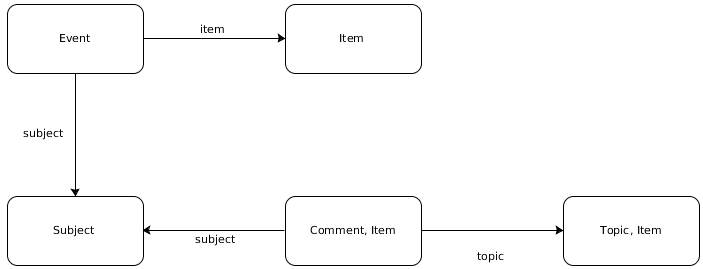
\includegraphics[width=.8\textwidth]{img/graph-model.png}
  \caption{Graph data model}
  \label{fig:graph-model}
\end{figure}

\subsubsection{Neo4j implementation}
\label{subsubsec:neo4j-implementation}

The physical data model for Neo4j is implemented using the community-supported Neo4j.rb library, which provides Ruby and Ruby on Rails bindings to the data store \autocite{Neo4jrb2010}.

The models developed during this research are available in \cref{ch:source-code}.

\section{Reference queries}
\label{sec:reference-queries}

In order to perform an empricial analysis on the selected data stores and the proposed physical data models, we present five reference queries in this chapter.
These reference queries will reflect the method of querying that would be the most common in the physical platform implementation, and mirrors the way data is queried from a database perspective.
All reference queries will be implemented using the available language bindings, however the generated implementation-specific query will also be presented.

Since the data of the use case is aimed at a write-once, read-many character, the majority of queries will not touch the data itself, but rather only read it.
Four read-only queries are included in the following sections, and one query that will insert new data into the data store.

\subsection{Querying}
\label{subsec:querying}

\subsubsection{Query 1}
\label{subsubsec:query-1}

``
Select N most recent events, ordered reverse chronologically
''

This query, as most simple reference query presented, is an example of a query that can be used on the homepage of the platform.
When a user opens the web application, a reverse chronologically ordered list of events is presented.
This view allows for a quick overview of the activity in the platform, and since the user is not signed in yet, it is not tailored.
This also means that everyone who visits the platform without signing in will receive the same events in their Recent Activity feed.

\subsubsection*{MongoDB}

\begin{listing}[H]
  \begin{minted}{ruby}
  MongoDB::Event
    .all
    .order_by(:created_at => :desc)
    .limit(count)
    .each(&:to_s)
  \end{minted}

  \caption{MongoDB query 1}
  \label{lst:mongodb-query-1}
\end{listing}

\subsubsection*{Neo4j}

\begin{listing}[H]
  \begin{minted}{ruby}
  Neo4j::Event
    .all
    .order(:created_at => :desc)
    .limit(count)
    .each(&:to_s)
  \end{minted}

  \caption{Neo4j query 1}
  \label{lst:neo4j-query-1}
\end{listing}

\begin{listing}
  \begin{minted}{cypher}
  MATCH (result_neo4jevent:`Event`)
    RETURN result_neo4jevent
    ORDER BY result_neo4jevent.created_at DESC
    LIMIT {limit_1} | {:limit_1=>count}

  MATCH (previous:`Event`)
    WHERE (ID(previous) = {ID_previous})
    OPTIONAL MATCH (previous)-[rel1:`by`]->(next:`Subject`)
    RETURN
      ID(previous),
      collect(next) | {:ID_previous=>result_neo4jevent.id}

  MATCH (previous:`Event`)
    WHERE (ID(previous) = {ID_previous})
    OPTIONAL MATCH (previous)-[rel1:`on`]->(next:`Item`)
    RETURN
      ID(previous),
      collect(next) | {:ID_previous=>result_neo4jevent.id}
  \end{minted}

  \caption{Neo4j query 1 (CYPHER)}
  \label{lst:neo4j-query-1-cypher}
\end{listing}

The Neo4j ORM call get converted into three distinct queries: one to get the \texttt{Event} node and two queries to get the related nodes \texttt{Subject} and \texttt{Item}.

\subsubsection{Query 2}
\label{subsubsec:query-2}

``
Select N most recent events, where the event is related to a topic in a list of given topics, ordered reverse chronologically
''

A user has to ability to subscribe to topics, which means that the Recent Activity feed may be tailored to the user.
Once the user logs in to the platform, the Recent Activity feed can be presented in a more attractive way.
The events in the feed will then consist of only events related to topics the user has subscribed to (which also includes the topics where the user is author or contributor).

\subsubsection*{MongoDB}

\begin{listing}[H]
  \begin{minted}{ruby}
  # List of subscribed topic identifiers
  topic_ids = [...]

  MongoDB::Event
    .in('item._id' => topic_ds)
    .order_by(:created_at => :desc)
    .limit(count)
    .each(&:to_s)
  \end{minted}

  \caption{MongoDB query 2}
  \label{lst:mongodb-query-2}
\end{listing}

\subsubsection*{Neo4j}

\begin{listing}[H]
  \begin{minted}{ruby}
  # List of subscripted topic identifiers
  topic_ids = [...]

  Neo4j::Topic
    .where(:id => topic_ids)
    .events
    .order_by(:created_at => :desc)
    .limit(count)
    .each(&:to_s)
  \end{minted}

  \caption{Neo4j query 2}
  \label{lst:neo4j-query-2}
\end{listing}

\begin{listing}[H]
  \begin{minted}{cypher}
  MATCH (node2:`Topic`:`Item`)
    WHERE (node2.uuid IN {node2_uuid})
    MATCH (node2)<-[rel1:`on`]-(result_events:`Event`)
    RETURN result_events
    ORDER BY result_events.created_at DESC
    LIMIT {limit_1} | {:limit_1=>1, :node2_uuid=>topic_ids}

  MATCH (previous:`Event`)
    WHERE (ID(previous) = {ID_previous})
    OPTIONAL MATCH (previous)-[rel1:`by`]->(next:`Subject`)
    RETURN
      ID(previous),
      collect(next) | {:ID_previous=>node2.id}

  MATCH (previous:`Event`)
    WHERE (ID(previous) = {ID_previous})
    OPTIONAL MATCH (previous)-[rel1:`on`]->(next:`Item`)
    RETURN
      ID(previous),
      collect(next) | {:ID_previous=>node2.id}
  \end{minted}

  \caption{Neo4j query 2 (CYPHER)}
  \label{lst:neo4j-query-2-cypher}
\end{listing}

\subsubsection{Query 3}
\label{subsubsec:query-3}

``
Select N most recent events, where the event is related to a given topic, ordered reverse chronologically
''

Every topic also has an overview page, which mainly contains metadata such as description, author, contributors and other information not directly related to the course content.
Next to the metadata, a custom Recent Activity feed is also included on the page.
This feed only contains events related to the topic the user is currently viewing, and effectively presents a timeline of changes and discussions.

\subsubsection*{MongoDB}

\begin{listing}[H]
  \begin{minted}{ruby}
  # Topic identifier
  topic_id = ...

  MongoDB::Event
    .where('item._id' => topic_id)
    .order_by(:created_at => :desc)
    .limit(count)
    .each(&:to_s)
  \end{minted}

  \caption{MongoDB query 3}
  \label{lst:mongodb-query-3}
\end{listing}

\subsubsection*{Neo4j}

\begin{listing}[H]
  \begin{minted}{ruby}
  # Topic identifier
  topic_id = ...

  Neo4j::Topic
    .find(topic_id)
    .events
    .order(:created_at => :desc)
    .limit(count)
    .each(&:to_s)
  \end{minted}


  \caption{Neo4j query 3}
  \label{lst:neo4j-query-3}
\end{listing}

\begin{listing}[H]
  \begin{minted}{cypher}
  MATCH (neo4j_topic)
    WHERE (ID(neo4j_topic) = {ID_neo4j_topic})
    MATCH (neo4j_topic)<-[rel1:`on`]-(result_events:`Event`)
    RETURN result_events
    ORDER BY result_events.created_at DESC
    LIMIT {limit_1} | {:limit_1=>1, :ID_neo4j_topic=>topic_id}

  MATCH (previous:`Event`)
    WHERE (ID(previous) = {ID_previous})
    OPTIONAL MATCH (previous)-[rel1:`by`]->(next:`Subject`)
    RETURN
      ID(previous),
      collect(next) | {:ID_previous=>neo4j_topic.id}

  MATCH (previous:`Event`)
    WHERE (ID(previous) = {ID_previous})
    OPTIONAL MATCH (previous)-[rel1:`on`]->(next:`Item`)
    RETURN
      ID(previous),
      collect(next) | {:ID_previous=>neo4j_topic.id}
  \end{minted}

  \caption{Neo4j query 3 (CYPHER)}
  \label{lst:neo4j-query-3 (CYPHER)}
\end{listing}

\subsubsection{Query 4}
\label{subsubsec:query-4}

``
Select N most recent events, where the event is related to a given user, ordered reverse chronologically
''

Similarly to topics, a profile page also includes a timeline of the user's activities: additions, deletions, comments and annotations that were recently made by that user.

\subsubsection*{MongoDB}

\begin{listing}[H]
  \begin{minted}{ruby}
  # Subject identifier
  subject_id = ...

  MongoDB::Event
    .where('subject._id' => subject_id)
    .order_by(:created_at => :desc)
    .limit(count)
    .each(&:to_s)
  \end{minted}

  \caption{MongoDB query 4}
  \label{lst:mongodb-query-4}
\end{listing}

\subsubsection*{Neo4j}

\begin{listing}[H]
  \begin{minted}{ruby}
  # Subject identifier
  subject_id = ...

  Neo4j::Subject
    .find(subject_id)
    .events
    .order(:created_at => :desc)
    .limit(count)
    .each(&:to_s)
  \end{minted}

  \caption{Neo4j query 4}
  \label{lst:neo4j-query-4}
\end{listing}

\begin{listing}[H]
  \begin{minted}{cypher}
  MATCH (n:`Subject`)
    WHERE (n.uuid = {n_uuid})
    RETURN n
    ORDER BY n.uuid
    LIMIT {limit_1} | {:n_uuid=>subject_id, :limit_1=>1}

  MATCH (neo4j_subject)
    WHERE (ID(neo4j_subject) = {ID_neo4j_subject})
    MATCH (neo4j_subject)<-[rel1:`by`]-(result_events:`Event`)
    RETURN result_events
    ORDER BY result_events.created_at DESC
    LIMIT {limit_1} | {:limit_1=>1, :ID_neo4j_subject=>subject_id}

  MATCH (previous:`Event`)
    WHERE (ID(previous) = {ID_previous})
    OPTIONAL MATCH (previous)-[rel1:`by`]->(next:`Subject`)
    RETURN
      ID(previous),
      collect(next) | {:ID_previous=>result_events.id}

  MATCH (previous:`Event`)
    WHERE (ID(previous) = {ID_previous})
    OPTIONAL MATCH (previous)-[rel1:`on`]->(next:`Item`)
    RETURN
      ID(previous),
      collect(next) | {:ID_previous=>result_events.id}
  \end{minted}

  \caption{Neo4j query 4 (CYPHER)}
  \label{lst:neo4j-query-4}
\end{listing}

\subsection{Insertion}
\label{subsec:insertion}

\subsubsection{Query 5}
\label{subsubsec:query-5}

``
Insert N given :created or :updated events
''

Finally, since read requests will most likely outnumber write requests with several magnitudes in the studied use case, only one query where data is inserted is presented.
The query creates a single event in the data store.

\subsubsection*{MongoDB}

\begin{listing}[H]
  \begin{minted}{ruby}
  # Subject identifier
  subject_id = ...

  # Item identifier
  item_id = ...

  MongoDB::Event.create! :subject => subject_id,
                         :item => item_id,
                         :predicate => :updated
  \end{minted}

  \caption{MongoDB query 5}
  \label{lst:mongodb-query-5}
\end{listing}

\subsubsection*{Neo4j}

\begin{listing}[H]
  \begin{minted}{ruby}
  # Subject identifier
  subject_id = ...

  # Item identifier
  item_id = ...

  Neo4j::Event .create! :subject => subject_id,
                        :item => topic_id,
                        :predicate => :updated
  \end{minted}

  \caption{Neo4j query 5}
  \label{lst:neo4j-query-5}
\end{listing}

\begin{listing}[H]
  \begin{minted}{cypher}
  MATCH (n:`Subject`)
    WHERE (n.uuid = {n_uuid})
    RETURN n
    ORDER BY n.uuid
    LIMIT {limit_1} | {:n_uuid=>subject_id, :limit_1=>1}

  MATCH (n:`Item`)
    WHERE (n.uuid = {n_uuid})
    RETURN n
    ORDER BY n.uuid
    LIMIT {limit_1} | {:n_uuid=>item_id, :limit_1=>1}

  CREATE (n:`Event`)
    SET n = {props}
    RETURN n | {:props=>{:uuid=>event_id, :created_at=>1526737892, :predicate=>1}}

  MATCH (n:`Subject`)
    WHERE (n.uuid = {n_uuid})
    RETURN n
    LIMIT {limit_1} | {:n_uuid=>subject_id, :limit_1=>1}

  MATCH
      (from_node),
      (to_node)
    WHERE
      (ID(from_node) = {ID_from_node}) AND
      (ID(to_node) = {ID_to_node})
    CREATE (from_node)-[rel:`by` {rel_create_props}]->(to_node)
      | {:ID_from_node=>event_id, :ID_to_node=>subject_id, :rel_create_props=>{}}

  MATCH (n:`Item`)
    WHERE (n.uuid = {n_uuid})
    RETURN n
    LIMIT {limit_1} | {:n_uuid=>item_id, :limit_1=>1}

  MATCH
      (from_node),
      (to_node)
    WHERE
      (ID(from_node) = {ID_from_node}) AND
      (ID(to_node) = {ID_to_node})
    CREATE (from_node)-[rel:`on` {rel_create_props}]->(to_node)
      | {:ID_from_node=>event_id, :ID_to_node=>item_id, :rel_create_props=>{}}
  \end{minted}

  \caption{Neo4j query 5 (CYPHER)}
  \label{lst:neo4j-query-5-cypher}
\end{listing}

\section{Conclusion}
\label{sec:data-model-conclusion}

In this chapter we presented an introduction to the domain, and provided some examples of events in the Recent Activity feed.
Futhermore, we analyzed this domain description, and derived a logical data model for both document- and graph-oriented data stores.
Next, we proposed an implementation of this logical data model for two document-oriented, and one graph-oriented data store in the Ruby language bindings available for the respective database management systems.
Finally, we presented five reference queries for the three data stores, and included both a language binding-specific DSL and a physical query implementation for each.

% TODO: Conclusion about ORMs

\chapter{Empirical study}
\label{ch:empirical-study}

In this chapter we will implement the previously proposed physical data models for the MongoDB, CouchDB and Neo4j data stores.
In this context, a Ruby on Rails application was developed that uses three libraries that provide language bindings to the respective data stores.
% TODO: references
A custom benchmarking framework was implemented using the RSpec library to provide structure and maintainability and the \texttt{Benchmark} class built into the Ruby implementation to measure query execution.

\section{Testing setup}
\label{sec:testing-setup}

In order to keep the results of the tests consistent, the following rules are applied:

\begin{itemize}
  \item Query caching is disabled
  \item Connection pooling is disabled
  \item Clustering is disabled
  \item No additional performance tweaks were applied on the database management systems
  \item All disk persistence is mapped to memory on a RAM disk, transparent to the database management systems
\end{itemize}

Native protocols were chosen for every data store: Mongo Wire Protocol for MongoDB, HTTP for CouchDB and Bolt for Neo4j.

All benchmarks were performed on a single machine with the following specifications:

\begin{itemize}
  \item Intel Core i7-3840QM (4 cores, 8 threads), 45W TDP
  \item Hyperthreading and \TODO{Intel Turbo Boost} enabled
  \item 32GB DDR4 RAM
  \item 180GB SATA-III SSD
\end{itemize}

The following software versions were used:

\begin{itemize}
  \item Arch Linux (rolling release)
  \item MongoDB 3.6.3
  \item CouchDB 2.1.1
  \item Neo4j Community Edition 3.0.6
  \item Ruby 2.5.0
\end{itemize}

\section{Procedure}
\label{sec:procedure}

In order to compare the performance of the three data stores, the following procedure was followed.

First, the database was filled with random testing data.
The amount of testing data linearly depends on a multiplication factor, which \TODO{varied} throughout the benchmark tests.

Next, the full test suite was ran sequentially for the three data stores, and the timing results were written to separate files.
It is important to note that every reference query was executed many times, depending on different factors.
Since the execution time of a single iteration is negligable, every query was executed a number of times to negate the effect of external factors, such as operating system scheduling and I/O wait times.
We have chosen the iteration counts of \TODO{1 000, 10 000 and 100 000}.
Having multiple iteration runs gives us the opportunity to analyze the vertical scalability of the query as well.
As indicated in the informal descriptions of the reference queries, the query itself is also dependent on a variable $N$ which signifies the event count that is to be retrieved from the database.
We believe a sane default for this value in a concrete implementation would be 100, meaning that 100 events will be retrieved on every query run.
However, in the test suite this variable takes the value of \TODO{100, 1 000 and 10 000} to allow for more reliable timings.

This gives us 9 timing results for every query for every data store in total.
These results are analyzed, graphed and discussed in the sections below.

\section{Previous work}
\label{sec:previous-work}

% Netflix benchmark, http://www.bgbenchmark.org/BG/, Yahoo! Cloud Serving Benchmark (YCSB)

\section{Conclusion}
\label{sec:comparative-study-conclusion}

\chapter{Opportunities}
\label{ch:opportunities}

Since the field of NoSQL is comprised of a lot of different products, varying in data model and features, choosing the right data store for a use case is a difficult and complex choice.
The analysis and comparison of the NoSQL data stores in this research has revealed certain pain points and opportunities for future research.

First, a common terminology needs to be established for NoSQL data stores, at least for data stores within the same NoSQL category that adhere to the same data model.
Comparing data stores using different vocabulary for the same concepts is confusing and impedes comparison and analysis of these products.
Establishing a common terminology in the NoSQL field will not only allow to make a more informed decision and doing this more efficient, but also facilitates the switch between different NoSQL products.

Secondly, the difficulty and time penalties imposed by the proposed implementation of the data models and reference queries in the three compared NoSQL data stores, proved that there certainly is an opportunity for a common querying language between NoSQL products, at least for data stores that have the same data model.
For example, the difference in interface between MongoDB's JavaScript API and CouchDB's REST API -- while still having the same data model -- does not allow for an easy switch between the two data stores, effectively requiring a complete rewrite and -engineering of the data storage layer in the application.
Standardizing the querying of NoSQL data stores -- at least per category -- would likely help the adoption of NoSQL storage systems and lower developer learning curve.

Some experimental solutions already exist to aggregate querying on certain data stores.
Hive provides an interface that uses SQL-like semantics to allow querying multiple data stores, however this project is in practice limited to a small number of backing stores, most importantly HBase and Cassandra \autocite{Hive2017}.
Another proposed solution is UnQL, a Unified Querying Language for NoSQL data stores \autocite{Buneman2000}.
This collaboration between Couchbase and SQLite aimed to implement a unified API covering all NoSQL data stores, from document-oriented to graph data stores.
However, seeing the massive scope of this project, it seems to have suffered from a severe case of hybris and is no longer being developed \autocite{Weinberger2012}.

There exists a similar discrepancy in data modeling for NoSQL data storage solutions.
Every product and more generally every NoSQL data store category imposes its own implementation-specific data modeling layer.
Since reimplementation and adjustment of the data storage layer of the application is a far reaching and costly operation, designing an application's data model for an intermediate, abstract data model before approaching the practical implementation would be a solution for this problem.
\citeauthor{Bugiotti2014} suggests a novel abstract data model for NoSQL systems called NoAM (NoSQL Abstract Model), which exploits certain commonalities between different NoSQL data models, allowing developers to model information in an intermediate format that can be adapted to multiple storage systems.

Additionally, RDF triple stores were not considered in the scope of this research.
However, similarly to key-value stores, usage of RDF semantics and the performance implications of data stores using simple data models may provide an interesting entrypoint for future research as an applied case study.

Finally, benchmarking NoSQL solutions is also a pain point encountered in this research.
There is no standardized way to provide reliable benchmarks of the different NoSQL categories, in part due to the data models that differ conceptually.
Any performance comparisons have to be done either at an atomic entity level, or a global use-case level as is presented in this thesis in order to obtain results that are reliable and not tainted by any modeling-specific conditions.
Furthermore, plenty of important factors were not considered in this research.
The performance benchmarks do not take into account the horizontal scalability of NoSQL solutions, and use the default configuration for each product.
Finetuning the database management system parameters would allow performance gains without any additional logical design or implementation.
Finally, since this thesis only represents a minor venture into NoSQL data modeling, the presented data models can also be improved upon.

% Opportunity: better Ruby ORM support for CouchDB
% Couchrest_model/mongoid: no enums
% TODO: dbms-specific features, such as mongodb capped collections; data expiration/TTL?
% TODO: indexing, sharding on date
% TODO: memcached?

%%=============================================================================
%% Conclusie
%%=============================================================================

\chapter{Conclusion}
\label{ch:conclusion}

%% TODO: Trek een duidelijke conclusie, in de vorm van een antwoord op de
%% onderzoeksvra(a)g(en). Wat was jouw bijdrage aan het onderzoeksdomein en
%% hoe biedt dit meerwaarde aan het vakgebied/doelgroep? Reflecteer kritisch
%% over het resultaat. Had je deze uitkomst verwacht? Zijn er zaken die nog
%% niet duidelijk zijn? Heeft het onderzoek geleid tot nieuwe vragen die
%% uitnodigen tot verder onderzoek?


% Result: Mongo
% Couch not supported
% Neo too slow
% Neo also acid, don't need that

% non-linked/embedded nature of mongodb increases performance massively


%%=============================================================================
%% Bijlagen
%%=============================================================================

\appendix

%%---------- Onderzoeksvoorstel -----------------------------------------------

\chapter{Research proposal}
\label{ch:research-proposal}

The subject of this thesis is based upon a research proposal that was graded by the promotor in advance. This proposal has been included as an attachment.

% Verwijzing naar het bestand met de inhoud van het onderzoeksvoorstel
%---------- Inleiding ---------------------------------------------------------

\section{Introduction} % The \section*{} command stops section numbering
\label{sec:introduction}

% problem and context
% motivation, relevance for the research
% goal and research questions

The \textcite{OpenWebslides} project provides a user-friendly platform to collaborate on webslides - slides made with modern web technologies such as HTML, CSS and JavaScript. One of the core features this application provides is \emph{co-creation}. The co-creation aspect manifests itself in several forms within the application; annotations on slides and a change suggesting system resembling GitHub's pull request feature are the main mechanisms. Because of the inherent social nature of co-creation, a basic notifications feed was also implemented. This feed is tailored to the user, and reflects the most recent changes, additions and comments relevant to the slide decks the user is interested in.

However, at the moment the functionality implemented in the system contains only the bare necessities. The module will be expanded in the future, and doing so requires a structural and conceptual rethinking of how the notifications are generated, stored and queried. The size of the dataset is also expected to grow linearly with user activity, therefore scalability is a requirement as well.

This paper has two research questions.

\begin{enumerate}
	\item What frameworks and software packages currently exist in the industry to store structured non-relational graph or document data?
	\item How is the social graph provided by the Open Webslides' notification feed structured and how is this data consumed?
\end{enumerate}

Answering these questions is paramount for the final section of the paper, which describes a data storage mechanism that performs well given the functional requirements of the project's data flow.

%---------- Use case ----------------------------------------------------------

\section{Use case}
\label{sec:use-case}

This thesis is a study of NoSQL data storage techniques applied to the \textcite{OpenWebslides} project. The online, interactive platform that the project provides includes a list of notifications in reverse chronological order, tailored to the user. This feature is called the \textit{social feed}. It enumerates the most recent social activity on the platform. For example, if a user updates a slide deck, the user's friends would be able to find a change notification in their respective social feeds.

From the perspective of the application code that generates the social feed, the user, slide deck and notification should be considered separate entities. The notification itself has relations to the other entities: the author (the \textit{subject}), the slide deck (the \textit{object}), along with the \textit{predicate} property that provides information on what operation was performed (for example creating or updating a slide deck).

This data model is also characterized by the \textit{write-once read-many} nature of the information; once the notification has been generated, it does not need to be modified again. It will also only be queried in a very specific way: the application server will always attempt to retrieve the most recent notifications starting from the user entity.
This principle is an important aspect to take into consideration in the choice of data storage mechanism.

%---------- Stand van zaken ---------------------------------------------------

\section{State-of-the-art}
\label{sec:state-of-the-art}

In current literature, studies such as \textcite{Moniruzzaman2013}, \textcite{NayakPoriyaPoojary2003} and \textcite{HammesMederoMitchell2014} have already analyzed the disparity between traditional relational database systems and NoSQL stores.
However, the conceptual and technical difference between these data storage models will not be scrutinized any further, since this paper presents a data storage solution applied to the social notification feed of the \textcite{OpenWebslides} project.

There are already many existing free and commercial products for the storage of NoSQL data, such as Redis \autocite{Redis}, CouchDB \autocite{CouchDB}, MongoDB \autocite{MongoDB} and Neo4j \autocite{Neo4j}. Finding the right database model for this use case (section \ref{sec:use-case}) is one of the hurdles this paper intends to handle. \textcite{Zhao2015} describes the development of a messaging system for astrophysical transient event notifications. Part of this paper is a qualitative comparison between document-based NoSQL storage solutions fit for this particular use case. We expect this paper to provide a solid base of reasoning in order to find a scalable and efficient solution for resolving similar computational challenges.

The goal of this paper is to provide a performant, scalable and maintainable data storage schema for the \textcite{OpenWebslides} platform, regarding the linked social graph that powers the \textit{Social Feed} functionality present in the platform.

% \autocite{KEY} => (Author, year)
% \textcite{KEY} => Author (year)

%---------- Methodologie ------------------------------------------------------
\section{Methodology}
\label{sec:methodology}

First, a range of industry-standard NoSQL database management systems such as MongoDB \autocite{MongoDB}, HBase \autocite{HBase} and Neo4j \autocite{Neo4j} will be qualitatively analyzed. Three of the five types of NoSQL database types \autocite{NayakPoriyaPoojary2003} will be included in the study: column-oriented, document based and graph databases. Criteria for comparison include how the database management system concretely stores its data on disk, the query format and specific programming language bindings. Another important aspect is the distributed nature of many NoSQL databases. Using Brewer's conjecture \autocite{Brewer2002} -- often called the CAP theorem -- the existing types of data storage systems will be examined and summarized. There is also a practical factor present in the research; this includes the license of the project, its active maintainability and future prospects.
Common types of NoSQL databases include key-value store, column-oriented, document store and graph databases \autocite{NayakPoriyaPoojary2003}. This paper will provide a short introduction to these types, before proceeding with the type that fits our use case the most.

Second, the data model specific to the Open Webslides project will be examined. We will start from the data model that is already implemented in the current iteration of the platform. At the time of writing, the existing base implementation of the social notification feed only contains two types of notifications. This paper will try to extrapolate this concept into a more generalized, abstract system in which developers can easily plug additional notification types.
The physical properties of the data model will also be taken into account: the data will be written to the data storage only once, but read many times. It is also highly interlinked information, as a notification will always relate to one or more users as a subject, and a target object as well -- most likely a slide deck or collection of slide decks. These links need to be maintained, and efficiently reconstructed when queried.

Finally, a sample dataset will be constructed using the aforementioned detailed analysis. Empirical testing will be conducted against multiple database management systems, and the results will be summarized and interpreted. Various information flows will be tested; however, the most important process remains efficiently querying the stored data.

Using the comparative study of storage engines, data model analysis and the empirical results an implementation plan will be constructed. This plan will serve as a recommendation for future development.

%---------- Verwachte resultaten ----------------------------------------------
\section{Expected results and conclusions}
\label{sec:expected_results_and_conclusions}

The NoSQL ecosystem, unlike relational databases, is headed towards specialization, so different solutions are headed in different directions \autocite{Maroo2013}. In this paper, we expect to find one type of NoSQL database that is a better fit for the Open Webslides use case, in clear contrast with the other types of storage engines. Due to the inherently highly interlinked nature of the stored data, we suspect a graph-based database management system to provide most advantages, and generally the most performant experience.

This expectation is amplified by the availability and good community support of Ruby bindings to the most popular graph database management systems.

Since the platform being discussed only caters to a small to medium user base, we do not expect the need to scale horizontally beyond one instance. However, the vertical scalability is still a topic for discussion, and we expect to determine the computational order of magnitude in order to efficiently query the given dataset during this study.

Finally, the implementation plan should describe a concrete roadmap, stretching over a development period with a baseline expectation of one to three months. Roll-out of this mechanism should also be included in this plan.

We also expect that this thesis will provide a good reference to a further stable, scalable and extendable implementation of the \textit{social feed} feature in the \textcite{OpenWebslides} project as outlined in section \ref{sec:use-case}.


%%---------- Andere bijlagen --------------------------------------------------
% TODO: Voeg hier eventuele andere bijlagen toe
%\input{...}

\chapter{Source code}
\label{ch:source-code}

\section{MongoDB}
\label{sec:source-mongodb}

\subsection*{Event}
\inputminted[baselinestretch=1,fontsize=\footnotesize]{ruby}{app/app/models/mongo_db/event.rb}

\subsection*{Comment}
\inputminted[baselinestretch=1,fontsize=\footnotesize]{ruby}{app/app/models/mongo_db/comment.rb}

\subsection*{Item}
\inputminted[baselinestretch=1,fontsize=\footnotesize]{ruby}{app/app/models/mongo_db/item.rb}

\subsection*{Subject}
\inputminted[baselinestretch=1,fontsize=\footnotesize]{ruby}{app/app/models/mongo_db/subject.rb}

\subsection*{Topic}
\inputminted[baselinestretch=1,fontsize=\footnotesize]{ruby}{app/app/models/mongo_db/topic.rb}

\clearpage{}
\section{CouchDB}
\label{sec:source-couchdb}

\subsection*{Event}
\inputminted[baselinestretch=1,fontsize=\footnotesize]{ruby}{app/app/models/couch_db/event.rb}

\subsection*{Item}
\inputminted[baselinestretch=1,fontsize=\footnotesize]{ruby}{app/app/models/couch_db/item.rb}

\subsection*{Subject}
\inputminted[baselinestretch=1,fontsize=\footnotesize]{ruby}{app/app/models/couch_db/subject.rb}

\clearpage{}
\section{Neo4j}
\label{sec:source-neo4j}

\subsection*{Event}
\inputminted[baselinestretch=1,fontsize=\footnotesize]{ruby}{app/app/models/neo4j/event.rb}

\subsection*{Comment}
\inputminted[baselinestretch=1,fontsize=\footnotesize]{ruby}{app/app/models/neo4j/comment.rb}

\subsection*{Item}
\inputminted[baselinestretch=1,fontsize=\footnotesize]{ruby}{app/app/models/neo4j/item.rb}

\subsection*{Subject}
\inputminted[baselinestretch=1,fontsize=\footnotesize]{ruby}{app/app/models/neo4j/subject.rb}

\subsection*{Topic}
\inputminted[baselinestretch=1,fontsize=\footnotesize]{ruby}{app/app/models/neo4j/topic.rb}

\clearpage{}
\section{Empirical study}
\label{sec:source-empirical-study}

\subsection*{Seeds}
\inputminted[baselinestretch=1,fontsize=\footnotesize]{ruby}{app/db/seeds.rb}

\subsubsection*{MongoDB}
\inputminted[baselinestretch=1,fontsize=\footnotesize]{ruby}{app/db/seeds/mongo_db.rb}

\subsubsection*{Neo4j}
\inputminted[baselinestretch=1,fontsize=\footnotesize]{ruby}{app/db/seeds/neo4j.rb}

\clearpage{}
\subsection*{Benchmark support}
\inputminted[baselinestretch=1,fontsize=\footnotesize]{ruby}{app/spec/support/benchmark.rb}


%%---------- Referentielijst --------------------------------------------------

\printbibliography[heading=bibintoc]
%\addcontentsline{toc}{chapter}{\textcolor{maincolor}{\IfLanguageName{dutch}{Bibliografie}{Bibliography}}}

\end{document}
